%% Journal manuscript — Elsevier elsarticle class
%% Target: Transportation Research Part D: Transport and Environment

\documentclass[review]{elsarticle}

\usepackage{amsmath,amssymb,amsfonts}
\usepackage{graphicx}
\usepackage{textcomp}
\usepackage{booktabs}
\usepackage{multirow}
\usepackage{url}
\usepackage{hyperref}
\usepackage{xcolor}

\journal{Transportation Research Part D}

% Relax float placement: review mode is double-spaced, so default float
% fractions defer every large figure to the end of the manuscript.
\renewcommand{\topfraction}{0.95}
\renewcommand{\bottomfraction}{0.95}
\renewcommand{\textfraction}{0.03}
\renewcommand{\floatpagefraction}{0.7}
\setcounter{topnumber}{3}
\setcounter{totalnumber}{5}

\begin{document}

\begin{frontmatter}

\title{Contrails cannot exist without flights: physics-informed contrail detection, tracking, and attribution in ground-based camera video}

\author[ec]{Ramon Dalmau\corref{cor1}}
\ead{ramon.dalmau-codina@eurocontrol.int}
\author[ec]{Gabriel Jarry}
\author[ec]{Philippe Very}
\cortext[cor1]{Corresponding author.}
\affiliation[ec]{organization={EUROCONTROL Innovation Hub},
                 city={Brétigny-Sur-Orge},
                 country={France}}

\begin{abstract}
A contrail cannot exist without a flight. We exploit this constraint by inverting the usual detect-then-attribute pipeline: instead of finding contrails in an image and asking which flight made them, we start from each flight and ask whether its contrail is visible. Aircraft positions from surveillance data and reanalysis wind fields feed a contrail lifecycle model that predicts where each flight's contrail should appear in a ground-based camera image---not at the aircraft's position, but where the wind has carried the plume. These predictions become spatial prompts that guide a video segmentation model to either outline the contrail or reject the prompt when nothing is visible. Because each prompt belongs to exactly one flight, the output mask carries the flight's identity by construction, and tracking across frames requires no re-identification. We compare prompt encodings of increasing physical richness: binary presence, age-weighted freshness, and suppression of competing flights. On the GVCCS ground-camera dataset, the richest design improves mAP$_{25:75}$ by 25\% over the binary baseline, reaches 96.2\% attribution precision, rejects empty prompts with an AUC of 0.97, and maintains detection across three-quarters of a contrail's visible lifetime on average. Video-level bootstrap confidence intervals confirm that the attribution and segmentation-quality gains are statistically robust.
\end{abstract}

\begin{keyword}
contrails \sep climate impact \sep deep learning \sep video segmentation \sep flight attribution
\end{keyword}

\end{frontmatter}

\section*{Highlights}
\begin{itemize}
\item Flight and weather data become prompts telling SAM2 where contrails should appear
\item Detection, tracking, and flight attribution collapse into one segmentation pass
\item Age-weighted prompts raise attribution precision from 89.0\% to 96.2\%
\item Empty prompts are rejected with AUC 0.97 (94.3\% TPR, 6.5\% FPR at threshold 0.5)
\item Video-level bootstrap confirms the attribution and quality gains are significant
\end{itemize}

% ============================================================================
\section{Introduction}

Commercial aircraft at cruise altitude produce condensation trails when hot exhaust mixes with the cold, dry air near the tropopause. Whether a contrail persists depends on atmospheric humidity: at relative humidity above ice saturation, ice crystals grow by deposition and the contrail can spread through wind shear into broad cirrus sheets that trap outgoing infrared radiation; below saturation, crystals sublimate within minutes. Recent assessments put aviation contrail forcing on par with cumulative CO$_2$ emissions from aviation~\cite{lee2021contribution, teoh2023global}.

The mitigation path is narrow but tractable. Only 2 to 10\% of flights produce most of the contrail climate impact~\cite{teoh2020mitigating}, because formation and persistence depend on atmospheric conditions that vary sharply with altitude and location. Small altitude adjustments---500 to 1,000~feet---on those specific flights could reduce aviation's warming contribution at negligible fuel cost. Identifying which flights to divert requires prediction models that forecast where persistent contrails form. But prediction alone is not enough: models depend on meteorological inputs (humidity, temperature, wind) that carry substantial uncertainty at cruise altitude, and their contrail formation and persistence criteria
remain difficult to validate at the individual-flight level at scale, with only limited validation exercises reported in the literature. Observational monitoring is the necessary complement. Without it, prediction models cannot be validated at the individual-flight level, avoidance maneuvers cannot be confirmed in real time, and the datasets needed to improve forecasts cannot be built. Such monitoring can draw on satellite imagery, which covers wide areas but at coarser resolution and with a time lag, or ground-based cameras, which capture contrails at higher resolution shortly after formation. In both cases, monitoring requires three tightly linked capabilities: detecting contrails in the imagery, tracking them across frames as they evolve, and attributing each contrail to the specific flight that produced it.

The coupling among these three tasks is the central difficulty. Detection must distinguish contrail pixels from natural cirrus, sun glints, and image artifacts---hard, because contrails evolve from thin bright lines when fresh into diffuse patches indistinguishable from natural cirrus within tens of minutes. Tracking must follow each contrail across frames as it drifts with the wind, spreads laterally, fragments behind clouds, and changes brightness with sun angle. Attribution must then determine which aircraft produced each detected contrail. None of these tasks is independent of the others: a missed detection in frame $t$ leaves the tracker with no boundary to follow, and that track is permanently broken. A tracking swap at a crossing point delivers a wrongly identified track to the attribution algorithm, which assigns the wrong flight---silently, with no indication that an error occurred. Detection errors corrupt tracking; tracking errors corrupt attribution.

Existing approaches treat these as a sequential pipeline~\cite{chevallier2023linear, sarna2025benchmarking}. A detector segments contrail pixels from visual appearance. A tracker links masks across frames by appearance similarity. An attribution algorithm then matches tracked shapes to advected flight paths. Each stage takes only its own inputs and passes results forward.

\begin{figure}[!tbp]
\centering
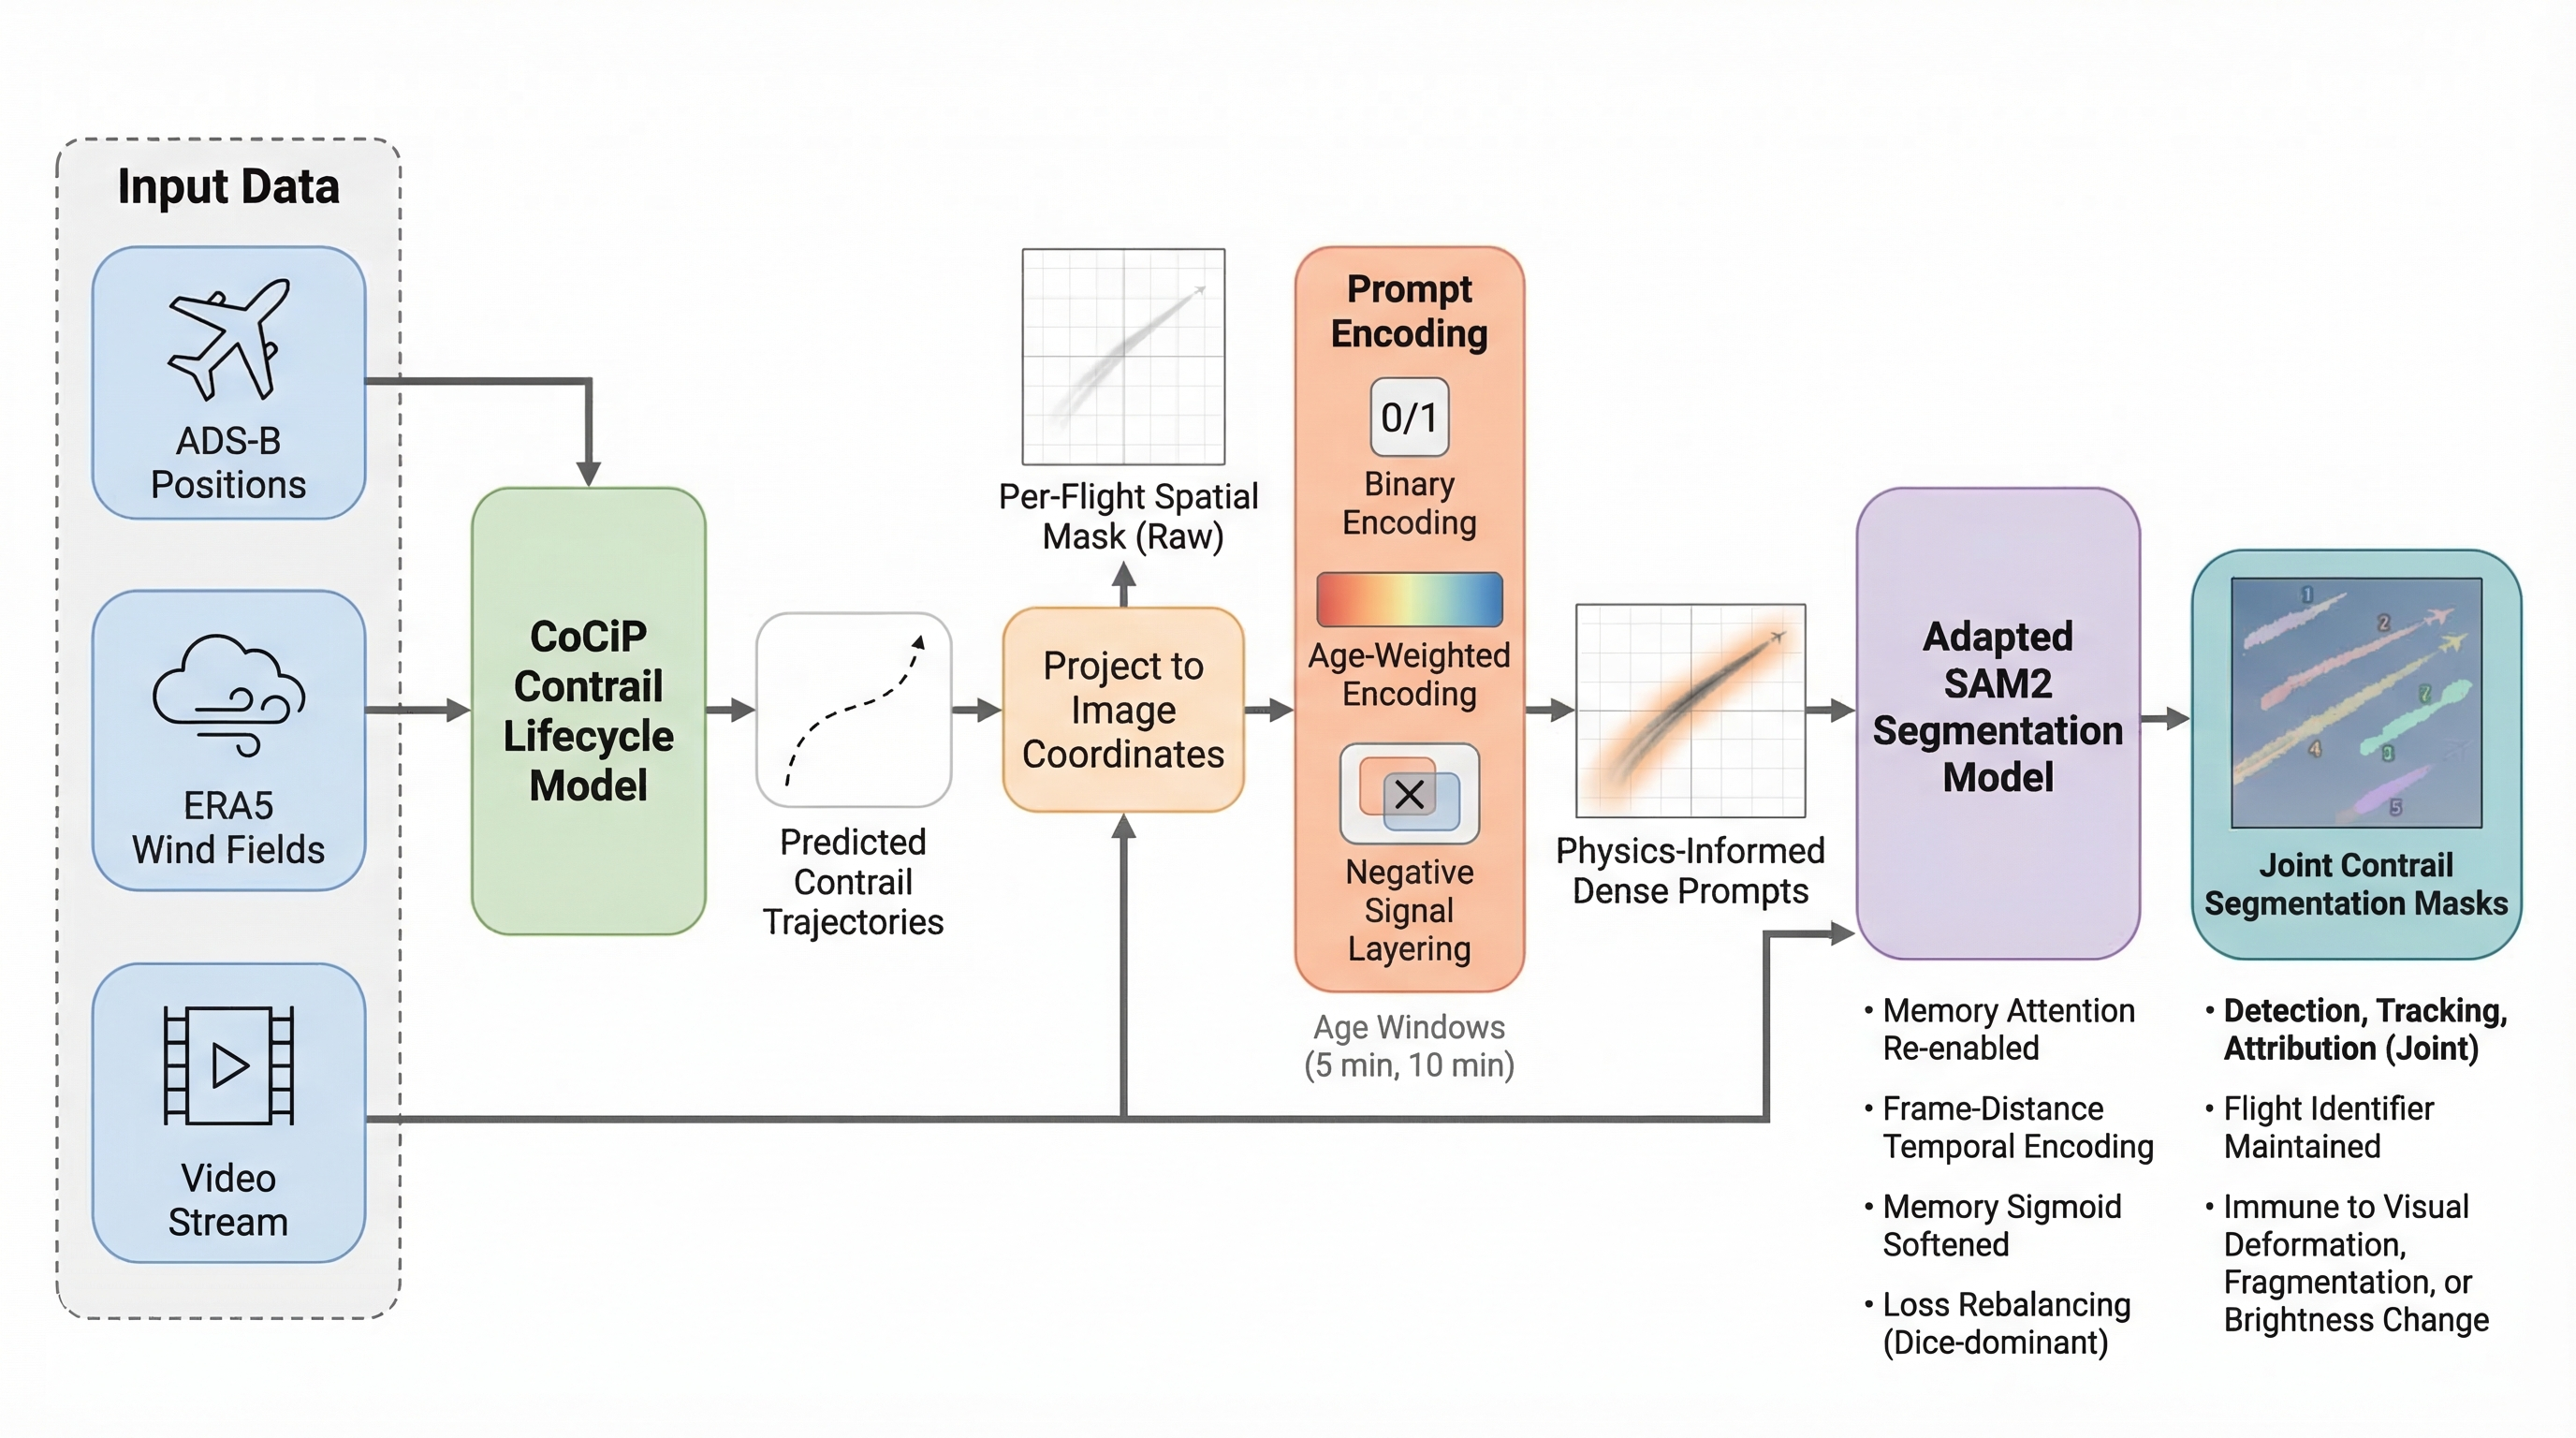
\includegraphics[width=\linewidth]{figures/fig_architecture.png}
\caption{System overview. ADS-B positions and ERA5 wind fields feed the CoCiP contrail lifecycle model, whose predicted trajectories are projected into image coordinates to produce per-flight spatial masks. Three prompt encodings are evaluated: binary (1-minute window), and age-weighted with or without negative-signal layering (5- and 10-minute windows). An adapted Segment Anything Model 2 (SAM2) model---with re-enabled memory attention, frame-distance temporal encoding, a softened memory sigmoid, dice-dominant loss rebalancing, and a disabled mask-decoder bypass---receives these dense per-frame prompts and outputs per-flight segmentation masks.}
\label{fig:system_overview}
\end{figure}

This one-way architecture has two structural problems. First, errors compound without recovery: a detection miss cannot be reversed by the tracker, and a tracking swap cannot be corrected by attribution. There are no feedback paths. Second, flight data enters the pipeline too late. Aircraft positions and wind fields are available from the start and could constrain the detector to search only where flights occurred---but in a sequential pipeline, this information is withheld until the final attribution stage, after detection and tracking are already done.

We address both problems by inverting the pipeline. Rather than detecting contrails and then attributing them, we start from flights and ask, for each one: does this flight's contrail appear in the image? Aircraft broadcast their positions via ADS-B (Automatic Dependent Surveillance-Broadcast). We combine these positions with wind and temperature fields from the ERA5 meteorological reanalysis~\cite{hersbach2020era5} and run the CoCiP contrail lifecycle model~\cite{schumann2012cocip} to predict where each flight's contrail should appear in the camera image. These predictions become spatial prompt masks that tell a video segmentation model where to look. The model---SAM2~\cite{ravi2024sam2}, adapted for dense per-frame prompting---either confirms the contrail with a refined segmentation mask or rejects the prompt with low confidence. The shift is from open-world detection (find all contrails anywhere in the scene) to constrained verification: physics specifies where to look, and the model decides what is actually there.

All three tasks follow directly. Detection is flight-aware: without a flight prompt, no output is generated for a location regardless of visual resemblance to a contrail. Tracking is implicit: each prompt carries a flight identifier across every frame, so no appearance-based association is needed; prompts follow atmospheric trajectories that remain geometrically consistent even when contrails deform, fragment, or cross. Attribution is by construction: each output mask corresponds to exactly one flight prompt.

A critical design choice underlies this inversion: we deliberately generate prompts for \emph{all} flights, including those for which the meteorological model predicts no contrail. Rather than filtering flights based on atmospheric pre-conditions, we let the visual model decide. This means the system must learn both confirmation (``the contrail is here, refine its boundary'') and rejection (``no contrail is visible despite the prompt, output nothing'')---a capability we call \emph{prompt rejection}. Prompt rejection is what makes the system safe to deploy without a thermodynamic pre-filter: uncertainty in ERA5 humidity is absorbed by the visual model rather than propagated as silent false rejections. Beyond the pipeline structure, we investigate how much physical information each prompt should encode---from flat binary presence masks to age-weighted encodings with suppression from competing flights. Section~\ref{sec:prompting} details the encoding strategies; Fig.~\ref{fig:system_overview} shows the full pipeline. Our contributions are:
\begin{enumerate}
    \item A framework that unifies contrail detection, tracking, and attribution into a single dense-prompting video segmentation task, with targeted modifications to SAM2's memory, temporal encoding, and loss for per-frame physics-derived prompts.
    \item A systematic comparison of prompt design along two axes---how much information each prompt pixel carries, and how far back in the contrail's life the prompt reaches. 
    \item An evaluation protocol that goes beyond standard segmentation metrics to assess the full detection--tracking--attribution chain: pixel-level quality across IoU thresholds, temporal tracking continuity and fragmentation, prompt discrimination, flight-level attribution precision, and cross-contamination between overlapping flights.
\end{enumerate}


% ============================================================================
\section{Background and Related Work}

This section covers contrail formation physics, surveys observational methods from satellite systems to ground cameras, and reviews related work on video object segmentation and contrail attribution.

\subsection{Contrail Formation and Climate Impact}
\label{sec:contrail_formation}

When jet engines burn kerosene at cruise altitude, the hot exhaust mixes with cold ambient air. The rapid cooling triggers condensation onto soot particles, forming ice crystals that scatter sunlight into visible white streaks. The Schmidt--Appleman criterion~\cite{schmidt1941entstehung, appleman1953formation, Schumann1996} defines the thermodynamic conditions under which contrails can form, depending on ambient temperature, humidity, and pressure. Whether a contrail persists depends on atmospheric humidity: if relative humidity exceeds 100\% with respect to ice, crystals grow by depositing water vapor from the surrounding air, allowing contrails to persist for hours and spread through wind shear into broad cirrus sheets. If humidity falls below this threshold, crystals sublimate and the contrail dissipates within minutes.

Persistent contrails evolve into contrail cirrus, artificial clouds that both reflect incoming solar radiation and trap outgoing infrared. For most contrails at typical cruise altitudes, the infrared warming effect dominates. The Contrail Cirrus Prediction model (CoCiP)~\cite{schumann2012cocip} simulates the full lifecycle of individual contrails, including ice crystal microphysics, radiative effects, and atmospheric dispersion. CoCiP divides each flight path into short segments and tracks each one forward in time: wind carries the segment's centerline, shear spreads it laterally, and microphysics governs ice crystal growth or sublimation. At any given moment, each segment has a known position, orientation, length, and width. We use this output to generate spatial prompts: the predicted contrail geometry is projected into camera image coordinates, producing a pixel-level map of where the contrail should appear. Section~\ref{sec:prompting} details the projection and encoding.

\subsection{Contrail Observation}
\label{sec:contrail_observation}

Contrails can be observed from satellites or ground cameras, each with distinct tradeoffs. Satellites cover wide areas and provide continuous monitoring~\cite{mannstein1999operational}, but young contrails are narrow and may fall below satellite pixel resolution. By the time contrails spread enough to be reliably detected from space, they have drifted far from the source aircraft, making attribution difficult because multiple flight paths intersect the contrail's current position. Machine learning has improved satellite detection~\cite{ng2023opencontrails}, but attribution remains challenging at satellite resolution.

Ground cameras~\cite{low2025ground, van2025contrail, jarry2025gvccs} capture sky images at higher spatial resolution and regular intervals, showing contrails shortly after formation when they remain near the source flight and attribution is more straightforward. The tradeoff is limited geographic coverage, weather dependency, and a fixed field of view. We use ground camera data because it provides unambiguous attribution ground truth: the camera catches contrails within minutes of formation, while the aircraft is still in or near the field of view, so the association between contrail and flight is geometrically unambiguous. The Ground-based Video Camera for Contrail Segmentation (GVCCS) dataset~\cite{jarry2025gvccs} provides the data for this work. It consists of sky image sequences captured at 30-second intervals from an all-sky camera at Br\'{e}tigny-sur-Orge, France, beneath European routes. Each contrail instance is annotated with multi-polygon masks that follow the contrail's shape across frames, linked to a unique flight identifier obtained from ADS-B records. The dataset is partitioned into training and test splits at the sequence level. Our test set contains 24 videos (4,781 frames). CoCiP generates prompts for the 3,432 flight--video pairs that crossed the camera's field of view during these sequences; of these, 610 produced visible contrails that were annotated with ground truth masks. The remaining 2,822 prompted flights have no visible contrail and serve as negative examples---the model must learn to reject them. Section~\ref{sec:dataset} provides further details on the training protocol.

\subsection{Segmentation and Video Object Segmentation}

Instance segmentation has progressed from encoder-decoder networks with skip connections~\cite{ronneberger2015u} to region-proposal methods~\cite{he2017maskrcnn} and transformer-based architectures like Mask2Former~\cite{cheng2021maskformer, cheng2021mask2former_video}, the last of which has been applied directly to video contrail segmentation~\cite{jarry2025gvccs} with strong per-frame accuracy but no built-in attribution.

For video object segmentation (VOS), memory-augmented approaches have become standard. XMem~\cite{cheng2022xmem} uses a multi-store memory system---working, sensory, and long-term banks updated online---enabling stable propagation over hundreds of frames. Cutie~\cite{cheng2024cutie} introduced object-level memory tokens that better handle occlusion and re-appearance. DeAOT~\cite{yang2022deaot} propagates associations hierarchically across feature scales. All of these assume sparse annotations: one or a few labeled frames anchor the track, and temporal memory carries it forward. None is designed to incorporate external domain knowledge that specifies object locations on every frame.

The Segment Anything Model (SAM)~\cite{kirillov2023sam} introduced promptable segmentation: given a point, bounding box, or rough mask, the model segments the indicated object without retraining. SAM2~\cite{ravi2024sam2} extends this to video by adding a temporal memory bank. The architecture has four parts: a vision backbone (Hiera~\cite{ryali2023hiera}) that extracts image features, a prompt encoder that converts the user's spatial input into a feature embedding, a memory bank that stores information from previously processed frames, and a mask decoder that combines all three to produce the final segmentation. In standard use, a human labels one or two \emph{conditioning frames}; SAM2 then propagates the segmentation through the remaining \emph{propagation frames} using the memory bank, without further human input. A thorough description of the SAM2 architecture is beyond the scope of this paper; readers seeking full architectural details are referred to the original publications~\cite{kirillov2023sam, ravi2024sam2}. Recent work has adapted SAM2 to a range of dense video understanding tasks, including camouflaged object segmentation~\cite{zhou2024sam2cos} and semantic segmentation~\cite{hesham2025sam2vss}; a broad survey of SAM2 adaptations is provided by Zhang and Tang~\cite{zhang2025sam2survey}. Our adaptation differs from these in that prompts are derived from a physics model external to the visual domain and provided on \emph{every} frame rather than propagated from sparse user annotations---to our knowledge the first SAM2 adaptation driven by per-frame, non-visual, physics-derived prompts.

Our setting reverses the typical ratio: every frame receives a physics-derived prompt, creating problems that SAM2 was not designed for. The modifications described in Section~\ref{sec:architecture} address these.

\subsection{Contrail Attribution}

Attribution algorithms match detected contrails to flights using geometric criteria~\cite{chevallier2023linear, riggi2023ai, geraedts2024scalable, dalmau2025attribution}. The general workflow projects aircraft trajectories into image coordinates, applies wind advection to account for drift between formation and observation, computes similarity metrics between detected shapes and predicted contrail locations, and solves an assignment problem. Chevallier et al.~\cite{chevallier2023linear} applied this approach to geostationary satellite data, matching linear features to advected flight paths. Riggi et al.~\cite{riggi2023ai} used probabilistic methods to handle uncertainty in both the detection and the trajectory projection. Geraedts et al.~\cite{geraedts2024scalable} developed a scalable system for large-scale satellite monitoring. Our previous framework~\cite{dalmau2025attribution} achieved high accuracy for young contrails using spatial and temporal consistency constraints from ground cameras. A common assumption across these works---including our own---is that detection and tracking are perfect: the attribution algorithm receives clean masks and unbroken tracks, so it can focus solely on the matching problem. In practice, detection and tracking are far from perfect, and errors in either stage propagate silently into attribution results. The present paper removes this assumption by evaluating the complete pipeline from raw images to flight-level attribution, with real (imperfect) detection and tracking.

All post-hoc methods share the structural limitation described in the introduction: flight information enters too late to help with segmentation, and errors propagate unchanged through the pipeline. Our approach eliminates this by making attribution intrinsic to the segmentation process.

% ============================================================================
\section{Flight-Conditioned Prompting}
\label{sec:prompting}

Every contrail traces back to an aircraft and a wind transport path. If we know where a flight occurred and how the wind carried the exhaust, we can predict where the resulting contrail should appear in the camera image. We exploit this to construct a spatial prompt for each flight on each frame: a pixel-level prediction of where that flight's contrail---not the aircraft itself, but the exhaust plume displaced by wind---should lie. How tight those prompts can be depends on how accurately we know the wind.

Prompt design is built up incrementally along two axes. The \emph{age window} $\tau_\text{max}$ sets how much of the contrail lifecycle to include: shorter windows give tighter localization; longer windows cover more of the visible track at lower spatial precision. The \emph{encoding richness} controls what each prompt pixel carries. The simplest encoding is binary (presence only). Age-weighted encoding adds a temporal gradient (intensity encodes contrail freshness). On top of the age-weighted encoding, a negative signal from competing flights can be layered. The two design axes---negative signal (absent vs.\ present) and age window---are independent: the negative signal formula applies at any window width, and the window choice does not alter the signal representation. Their contributions to segmentation quality are measured separately in Section~\ref{sec:results}.

Fig.~\ref{fig:prompt_comparison} illustrates the three encoding strategies on a scene with overlapping contrails. The window tradeoff is discussed under each encoding below; Section~\ref{sec:results} evaluates windows of 5 and 10~minutes.

\begin{figure}[!tbp]
\centering
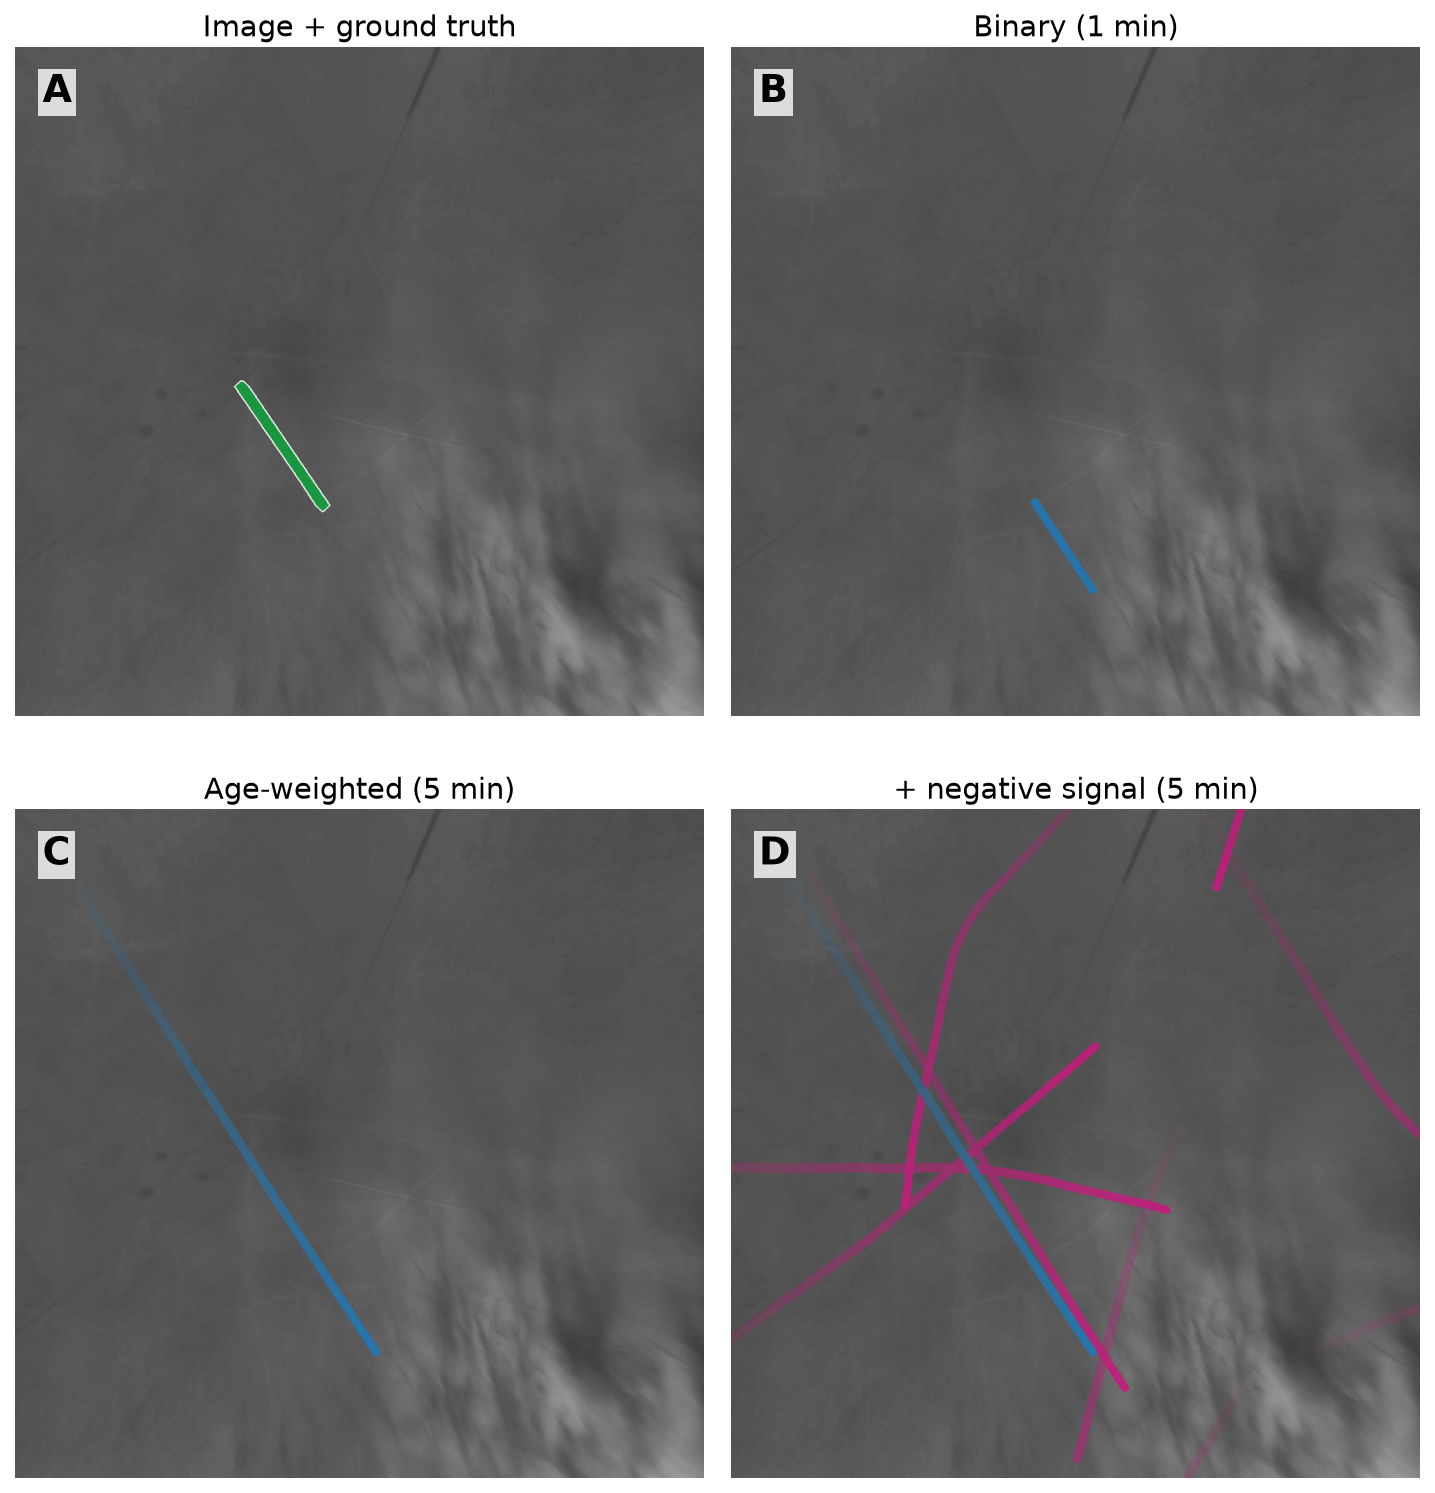
\includegraphics[width=\linewidth]{figures/fig_prompts.png}
\caption{The three prompt encodings on a real test-set flight (video~5, frame~104). (A)~Camera image with the ground truth annotation (green, thickened for visibility). (B)~Binary encoding: a flat presence mask restricted to the last minute of predicted geometry. (C)~Age-weighted encoding over a 5-minute window: intensity fades from bright (fresh, spatially reliable) to dim (old, potentially wind-drifted); note that the prompt extends beyond the annotated contrail---prompts are hints, not ground truth. (D)~Adding the negative signal: competing flights' predicted contrails (magenta) are layered as suppression; where they cross the target's own prompt (blue), the positive signal takes priority.}
\label{fig:prompt_comparison}
\end{figure}

\subsection{From Flights to Spatial Prompts}

Modern commercial aircraft broadcast their position continuously via ADS-B, transmitting GPS coordinates, barometric altitude, velocity vector, and a unique 24-bit ICAO identifier. Ground-based receivers collect these broadcasts into openly accessible databases such as the OpenSky Network~\cite{schafer2014opensky}, providing flight trajectory data for commercial air traffic.

We use \texttt{pycontrails}~\cite{pycontrails} to run CoCiP (Section~\ref{sec:contrail_formation}) on each flight's ADS-B trajectory with ERA5 meteorological fields~\cite{hersbach2020era5}. The output is a time series of contrail segment states: centerline position, along-track length, cross-track width, and depth.

Meteorological inputs come from two ERA5 products~\cite{hersbach2020era5}. Wind, temperature, specific humidity, vertical velocity, and cloud ice water content are retrieved on model levels covering the cruise altitude range. Contrails spread sideways because wind speed changes with altitude (wind shear), so getting the vertical wind profile right matters more than horizontal detail. Model levels are spaced more finely in altitude at cruise height than the standard pressure-level product. Radiation variables (surface shortwave and longwave fluxes) are retrieved separately. Both products have hourly temporal resolution, linearly interpolated to each segment's time. Table~\ref{tab:cocip_params} lists the CoCiP configuration parameters.

CoCiP transports each segment's centerline with the local wind velocity and models width growth through wake vortex dynamics in the first few minutes after formation, then diffusive spreading driven by atmospheric turbulence and wind shear. Aircraft-specific parameters (fuel flow, emissions index) are estimated by the Poll-Schumann performance model~\cite{poll2021estimation}. Integration uses a 30-second timestep to resolve the wake vortex phase, which shapes the contrail's initial geometry.

Two choices are critical for prompt generation and deserve particular attention. First, we deliberately disable both the Schmidt-Appleman formation filter and the initial-persistence filter. Standard CoCiP usage applies these filters to skip flights that are thermodynamically unlikely to form contrails, but ERA5 humidity at cruise altitude carries substantial uncertainty: the filters would reject some flights that do form visible contrails and pass some that do not. By running CoCiP on \emph{all} flights and generating prompts regardless of the meteorological prediction, we let the visual model decide whether a contrail is actually present. This design choice is what makes prompt rejection possible (Section~\ref{sec:results}): rather than relying on a meteorological pre-filter that can fail silently, the model learns to output low confidence when visual evidence is absent, providing an explicit signal of uncertainty. Second, we correct ERA5 humidity bias using histogram matching~\cite{pycontrails} rather than a constant scaling factor, which adjusts the full humidity distribution to match radiosonde observations and produces more realistic contrail width and persistence estimates.

These design choices also point toward a natural extension for future work. Currently, the spatial prompt encodes only contrail \emph{position}---whether a contrail should be present in a given pixel. ERA5 also provides local relative humidity, temperature, and wind shear, all of which govern contrail appearance and evolution. Embedding these scalar atmospheric fields directly in the prompt---for example, encoding humidity as a per-pixel intensity alongside the geometry mask---would give the model additional physical context at no labeling cost, potentially improving both detection confidence and boundary precision.



We convert CoCiP segment descriptions into two-dimensional image coordinates using the camera projection model described in~\cite{jarry2025gvccs}, with known intrinsic and extrinsic parameters calibrated for the all-sky camera. Each segment's spatial extent---a polygon in three-dimensional world coordinates---is projected into image coordinates to produce a prompt mask. The mask for a given flight is the union of all projected polygons from that flight's active segments.

\begin{table}[!tbp]
\centering
\caption{CoCiP configuration used for prompt generation, implemented with \texttt{pycontrails}~\cite{pycontrails}.}
\label{tab:cocip_params}
\resizebox{\linewidth}{!}{%
\begin{tabular}{l l l}
\toprule
\textbf{Parameter} & \textbf{Value} & \textbf{Description} \\
\midrule
\multicolumn{3}{l}{\textit{Integration}} \\
\quad Integration timestep       & 30 s           & Captures wake vortex descent in first minutes \\\quad Max contrail age           & Video duration & Tracks contrails for the full observation period \\\quad SAC filter                 & Disabled       & All flights prompted; model learns to reject non-contrailing flights \\\quad Persistence filter         & Disabled       & Same rationale; ERA5 humidity too uncertain to pre-filter \\\midrule
\multicolumn{3}{l}{\textit{Meteorology \& aircraft}} \\
\quad Humidity scaling           & Histogram matching~\cite{pycontrails} & Distribution-corrected ERA5 humidity \\
\quad Performance model          & PSFlight~\cite{poll2021estimation}  & Fuel flow and emissions from flight parameters \\
\bottomrule
\end{tabular}}
\end{table}

\subsection{Prompt Encoding Strategies}

We evaluate three prompt encodings of increasing richness: binary, age-weighted, and age-weighted with a negative signal. All three use the same projected contrail geometry; they differ only in what information each pixel carries.

\paragraph{Binary prompts.} The simplest strategy is a binary mask: pixels inside predicted contrail polygons are set to 1, all others to 0. This matches SAM2's original mask prompt interface, where any nonzero region means ``look here.'' Binary prompts tell the model where a contrail should be but carry no information about how old the contrail is or how confident the prediction is.

For each video frame at time $t$, we restrict prompts to contrail geometry younger than a maximum age $\tau_\text{max}$. Three factors motivate a short window. First, wind errors accumulate over time: a prompt that is off by a few pixels at 1~minute may be off by tens of pixels at 10~minutes. Second, young contrails are thin, so prompt regions tightly match the real contrail width; older contrails have spread, producing wider prompts that give the model less spatial guidance. Third, fresh contrails are bright and high-contrast; older contrails fade, so prompting on young geometry aligns the spatial prior with the phase where visual evidence is strongest. However, a short window also has drawbacks: it may miss contrails that become visible only after a delay---for instance, when clouds initially obscure formation and the contrail emerges minutes later---and it cannot capture the full curvature of a contrail that has spread along a long wind-sheared path. A longer window covers more of the contrail's visible extent and catches late-appearing segments, at the cost of including older geometry that may have drifted from the actual contrail position. Section~\ref{sec:results} evaluates 5- and 10-minute windows for the age-weighted encodings; the binary baseline uses a 1-minute window.

\paragraph{Age-weighted prompts.} Binary prompts discard temporal information that could help the model. A contrail segment formed 30~seconds ago is visually bright and spatially well-localized; one formed 8~minutes ago is faint and may have drifted from the predicted position. We encode this by setting prompt pixel intensity proportional to contrail freshness:
\begin{equation}
    p(x, y) = 1 - \frac{a(x,y)}{\tau_\text{max}},
\label{eq:age_prompt}
\end{equation}
where $a(x,y)$ is the age of the contrail segment covering pixel $(x,y)$ in minutes. A segment that just formed has intensity~1.0; intensity decreases linearly with age, and segments at or beyond the age limit $\tau_\text{max}$ contribute no prompt signal. This encoding gives the model a prior on where the contrail should be brightest and most reliably localized, effectively encoding temporal confidence into the spatial signal.

The age-weighted encoding interacts with the window tradeoff described above: with a wider window, the gradient from bright (young, reliable) to dim (old, uncertain) lets the model discount the spatial precision of older segments rather than treating all prompt pixels equally.

\paragraph{Prompts with a negative signal.} When multiple flights produce nearby or overlapping contrails, the model may incorrectly segment one flight's contrail under another flight's prompt. Binary and age-weighted prompts encode only the target flight's predicted contrail location; they carry no information about other flights nearby. Adding a negative signal extends the age-weighted encoding by layering suppression from all other flights' prompts on top of the target flight's positive age-weighted prompt.

For each frame, we compute a union mask $u(x,y)$ that combines the age-weighted prompts of all flights in the scene. The prompt with negative signal for flight $k$ is:
\begin{equation}
    p_k(x, y) = \begin{cases}
        p_k^+(x, y) & \text{if } p_k^+(x, y) > 0 \\
        -u(x, y)    & \text{if } p_k^+(x, y) = 0 \text{ and } u(x,y) > 0 \\
        0            & \text{otherwise,}
    \end{cases}
\label{eq:neg_prompt}
\end{equation}
where $p_k^+$ is the age-weighted prompt for flight $k$ (Eq.~\ref{eq:age_prompt}). Positive values indicate ``your contrail should be here, with this confidence.'' Negative values indicate ``another flight's contrail is here, not yours.'' Zero means background. The positive signal has priority: where the target flight's prompt overlaps with others, the target flight wins. The negative signal is also age-weighted, so the model learns that a negative region with a fresh nearby contrail deserves stronger suppression than one with only old, diffuse contrails. In principle, the negative signal could also be binary (present/absent) rather than age-weighted; we tested only the age-weighted variant, which preserves the temporal gradient on both sides. This means the negative signal axis is not fully factorial: we did not train a binary-encoding + negative-signal variant, so we cannot isolate the negative signal's effect from the age-weighting with certainty.

The resulting prompt values lie in $[-1, 1]$ and are passed directly to SAM2's prompt encoder without rescaling. The prompt encoder's convolutional layers learn to map this range during fine-tuning: positive values activate the target flight's contrail region, negative values suppress competing flights, and zero represents uninformative background.

\subsection{Edge Cases}

Several situations require careful handling.

\paragraph{No contrail formed.} When atmospheric conditions did not satisfy the formation criterion, or the contrail formed but dissipated immediately in ice-subsaturated air, we still generate a prompt because formation prediction from ERA5 humidity data is uncertain. The model learns to reject such prompts when no visual evidence supports them. This converts contrail formation prediction from a meteorological problem into a visual recognition problem.

\paragraph{Fragmented contrails.} Turbulence can break a contrail into disconnected segments. Our prompt mask shows the complete predicted trajectory as a continuous region, but the model can produce a segmentation covering only the visible segments with gaps where the contrail fragmented. Identity is preserved because the prompt carries the flight identifier regardless of fragmentation.

\paragraph{Prompts are hints, not hard constraints.} The model does not segment exactly where the prompt says. Prompts tell the model approximately where to look, but the final segmentation boundary follows visual evidence in the image. In training, the ground truth mask is typically offset by several pixels from the prompt polygon---wind errors, projection inaccuracies, and the contrail's actual shape all contribute---so the model learns that prompts and ground truth do not align perfectly. At inference, it can deviate from the prompt when the image shows the contrail is slightly elsewhere, rather than blindly tracing the prompt boundary. The age-weighted encoding reinforces this: bright (young) prompt regions are spatially reliable and the model trusts them closely, while dim (old) regions may be displaced, and the model relies more on what it sees. Without this tolerance for prompt--contrail misalignment, the system would fail whenever ERA5 wind estimates are off by even a few meters per second.

\paragraph{Unprompted contrails.} Contrails that formed outside the camera's field of view and drifted into the observable region have no associated flight in our ADS-B data and are missed by design. This is not a practical limitation in the envisaged deployment. A network of cameras, each covering a different region of sky, would ensure that every contrail is young and promptable in at least one camera's field of view---the same contrail that appears as an old, unprompted feature in one camera was freshly formed and correctly attributed in another. Within each camera, our prompt-based model handles attribution for flights that cross the field of view, while a complementary open-world detection model (e.g., Mask2Former~\cite{jarry2025gvccs}) could flag contrail-like features that lack a prompt as a consistency check.

% ============================================================================
\section{Model Architecture and Training}
\label{sec:architecture}

We build on SAM2.1~\cite{ravi2024sam2} with the Hiera Base+ backbone~\cite{ryali2023hiera}, pretrained on SA-V. Standard SAM2 expects a human to annotate one or two frames, then propagates the segmentation through the video using a memory bank. Replacing those annotations with physics-derived mask prompts on every frame violates three SAM2 defaults---in the training loop, memory mechanism, and loss function---each of which we modify below.

\subsection{Dense Prompt Training Loop}

SAM2's training loop is designed for sparse human annotations: it samples one or two initial conditioning frames where the user provides a click or mask, then propagates to the remaining frames using predicted masks alone. Conditioning frames receive the prompt directly and skip the memory-based decoder; propagation frames rely entirely on temporal memory from previous predictions. This sparse-annotation assumption runs deep: it determines how the memory bank is populated, which frames query temporal context, and how the decoder is invoked. Replacing sparse human annotations with dense physics-derived prompts on every frame breaks it entirely. There are no propagation frames, every frame is a conditioning frame, and the training loop must be restructured accordingly.

We replace the training loop with sequential processing. At each frame~$t$, the pipeline (1)~encodes the image through Hiera~B+ to extract multi-scale visual features at resolutions from $1/4$ to $1/32$, (2)~encodes the flight's prompt mask into a dense feature embedding through the prompt encoder, (3)~queries the memory bank via cross-attention to retrieve temporal context from previous frames, and (4)~decodes a segmentation mask and object score through the mask decoder. The resulting features and predicted mask are stored in the memory bank before advancing to frame~$t{+}1$. This means every subsequent frame can attend to all previous predictions, building up temporal context incrementally rather than propagating from a single reference.

We also disable a default where mask inputs bypass the decoder. In interactive use, the user's mask is already close to the ground truth and SAM2 copies it directly to the output, skipping the decoder for efficiency. Our prompt masks define where to look, not the exact object boundary---they are coarse physics predictions based on advection modeling, typically offset by a few pixels from the actual contrail edge and smoothed by the polygon rasterization process. Forcing every frame through the full mask decoder ensures that the final segmentation follows actual image evidence (the contrail's visual boundary) rather than the prompt geometry (the advection model's predicted polygon).

The distinction matters quantitatively. When the decoder bypass is active, the model copies the prompt geometry as the output mask, so IoU with ground truth is determined entirely by prompt accuracy rather than visual segmentation. The mask decoder, informed by Hiera visual features, refines prompt geometry into the higher IoU values reported in Table~\ref{tab:ablation}.

\subsection{Memory Adaptations}

Three SAM2 defaults assume sparse interactive conditioning and fail under dense prompting.

\paragraph{Memory attention for conditioning frames.} Standard SAM2 skips memory attention for conditioning frames, since the user already provided a correct mask and temporal context is unnecessary. When every frame is a conditioning frame, no frame queries memory and temporal propagation stops entirely. We re-enable memory attention for conditioning frames, limiting it to the 5 most recent to keep computation tractable on long sequences. This allows each frame to benefit from context about what the model has seen and predicted in previous frames, even when a fresh prompt is available.

\paragraph{Temporal position encoding.} Standard SAM2 assigns all conditioning frames temporal position zero, treating them as timeless reference anchors. With one or two reference frames among many propagation frames, this is fine. With dense conditioning, every frame gets position zero and the model cannot distinguish recent from distant context. We assign positions based on actual frame distance, so the model knows whether a memory entry is from one frame ago or twenty.

\paragraph{Memory sigmoid.} SAM2 converts predicted mask logits to memory features through a sigmoid with scale~20 and bias~$-10$. At scale~20, a logit of $0.3$ maps to $\sigma(20 \times 0.3 - 10) = \sigma(-4) \approx 0.02$, effectively zero. Memory is stored at $64 \times 64$ resolution ($1/16$ of the $1024 \times 1024$ input), so a contrail 2--4~pixels wide in the original image covers 0.1--0.25 memory pixels. Partial coverage produces logits near 0.1--0.3, which the hard sigmoid maps to near zero---erasing the contrail from temporal context before the next frame can query it. We use scale~1 and bias~0, which acts as a near-linear mapping near the origin, retaining partial values so the memory can encode ``thin structure here at $\sim$20\% confidence'' rather than ``nothing.'' Frames that cross-attend to this memory receive a valid, non-zero thin-structure signal from previous predictions.

The memory bank itself retains SAM2's default capacity (7 stored masks and 16 object pointers); only the cross-attention window over conditioning frames is restricted, to the 5 most recent. At the GVCCS temporal resolution of 30~seconds per frame, these 5 frames span 2.5~minutes of real time---enough to cover the period during which a contrail's appearance changes gradually and temporal context is most informative. Beyond this horizon, contrail morphology evolves substantially (spreading, fading, fragmenting), so older entries provide diminishing returns. The restriction also lowers GPU memory requirements, enabling training on longer sequences within hardware constraints. With more GPU memory, a wider attention window could help at higher frame rates, but 5 conditioning frames are sufficient at the GVCCS 30-second cadence.

\subsection{Loss Rebalancing for Thin Structures}

The total loss per frame combines four terms:
\begin{equation}
    \mathcal{L} = \lambda_\text{dice}\,\mathcal{L}_\text{dice} + \lambda_\text{focal}\,\mathcal{L}_\text{focal} + \mathcal{L}_\text{IoU} + \mathcal{L}_\text{cls}
\label{eq:loss}
\end{equation}
where $\mathcal{L}_\text{dice}$ is the dice loss on the predicted mask, $\mathcal{L}_\text{focal}$ is the per-pixel focal loss~\cite{lin2017focal}, $\mathcal{L}_\text{IoU}$ is the L1 loss on predicted IoU, and $\mathcal{L}_\text{cls}$ is the focal loss on the object score.

Contrails are thin: a typical contrail covers less than 0.1\% of the image pixels. SAM2's default loss weights focal at $\lambda_\text{focal}=20$ and dice at $\lambda_\text{dice}=1$. Focal loss sums over every pixel, so background pixels dominate the gradient. Dice loss normalizes by the mask area, giving thin objects and large objects equal weight. With the default weighting, the easiest way for the model to reduce total loss is to predict nothing---background focal loss drops to near zero, and the small dice penalty from missing a thin contrail is negligible. We invert the weights to $\lambda_\text{dice}=5$ and $\lambda_\text{focal}=1$ (chosen by manual iteration on training convergence, not grid search), and set focal $\alpha=0.75$ to up-weight the rare positive class. The area-normalized dice term now drives learning, with focal providing per-pixel boundary refinement rather than dominating the gradient.

Most flights crossing the camera do not produce visible contrails, so the model must learn to reject empty prompts. We supervise the object score head with focal loss ($\gamma=2$, $\alpha=0.75$), where $\alpha=0.75$ up-weights the rare ``object present'' class. When the object score predicts absence, the corresponding mask loss is still computed but the target mask is empty, so the model learns both ``nothing here'' and ``stop drawing pixels'' from the same negative examples.

\subsection{Dataset and Training Protocol}
\label{sec:dataset}

We use GVCCS~\cite{jarry2025gvccs}, the ground camera dataset described in Section~\ref{sec:contrail_observation}, with instance-level contrail annotations linked to flight identifiers. The camera captures sky images at 1024$\times$1024 resolution. Annotators labeled contrails with multi-polygon masks and unique identifiers persisting across frames. We partition at the sequence level to prevent information leakage.

We train without a held-out validation set, using all training sequences for learning. The dataset is small enough that holding out validation data would noticeably reduce the variety of contrail appearances and atmospheric conditions available for training. We instead select the number of training epochs per variant from training loss curves (Section~\ref{sec:training}). Early stopping on a validation metric would be more principled; we accept the less formal criterion in exchange for using all available training data.

\paragraph{Single-object lifecycle training.} Rather than training on clips with multiple overlapping flights, we train on one flight at a time. Each training sample follows a single flight's contrail through its full lifecycle: appearance, persistence, and disappearance. This simplifies learning because the model refines one prompt into one mask per sample without managing multi-object interactions. At inference time, SAM2's multi-object tracking processes multiple flights in parallel, but training benefits from reduced complexity. 

\paragraph{Object-centric sampling.} We treat each (video, flight) pair as a separate dataset entry. Within each epoch, every prompted flight is visited exactly once, regardless of how many frames it spans or whether the flight has ground truth masks. Many prompted flights have no visible contrail and therefore no ground truth---the model learns to reject these empty prompts as negative examples. A video with 15~prompted flights produces 15~training samples per epoch. This ensures short-lived contrails are sampled as frequently as long-lived ones, and negative examples are represented alongside positive ones.

\paragraph{Lifecycle sampler.} For each flight, the sampler discovers its temporal extent from the filesystem: first frame with a prompt mask, last frame with either prompt or ground truth. Sampling starts at the first prompt frame and takes every second frame (stride~2), so 13~model frames cover 26~real frames. Ideally, training would use consecutive frames to maximize temporal resolution, but GPU memory limits the sequence length that can be processed in a single forward pass. Using stride~2 doubles the real-time coverage per training sample while keeping memory requirements tractable, and we found that the 30-second inter-frame interval of GVCCS already provides smooth temporal context---skipping every other frame (60-second effective interval) still captures the gradual evolution of contrail appearance. Three additional frames are included past the last evidence of the contrail, teaching the model to output low scores and empty masks when visual evidence has vanished.

\paragraph{Augmentation.} Data augmentation must be applied consistently across the temporal dimension to preserve the physical relationships between frames. Random horizontal and vertical flips, random affine transforms (rotation $\pm 25^{\circ}$), and random grayscale (5\%) are applied with the same parameters across all frames in a sample. Critically, spatial transforms must also be applied to the prompt and ground truth masks, which have shape [H, W, 2] (channel~0 for ground truth, channel~1 for prompt). Color jitter is applied in two stages: a consistent pass across frames (brightness~0.1, contrast~0.03, saturation~0.03) simulates different sky lighting conditions, and an independent per-frame pass (brightness~0.1, contrast~0.05, saturation~0.05) mimics frame-to-frame illumination shifts from auto-exposure adjustments or passing clouds. The consistent jitter ensures the model sees the same ``sky'' across a training sample, while the independent jitter teaches robustness to short-term illumination changes that are common in ground camera sequences.

We deliberately omit ImageNet normalization. SAM2's pretrained checkpoint expects images normalized by ImageNet statistics, but ground camera sky images have very different statistics (dominated by blue and gray). During fine-tuning, we let the model adapt its internal normalization to the contrail domain. At inference, we override the default normalization with zero mean and unit standard deviation to match.

\paragraph{Optimization.} We fine-tune from the pretrained SAM2.1 checkpoint using AdamW~\cite{loshchilov2019adamw} with weight decay~0.1 (disabled for biases and LayerNorm parameters). The learning rate follows a 5\% linear warmup from $5 \times 10^{-7}$ to $5 \times 10^{-6}$, then cosine decay. The image encoder uses a lower peak rate of $3 \times 10^{-6}$ with layer-wise decay of~0.9 to preserve low-level features learned on the SA-V pretraining data. Training uses mixed-precision bfloat16, gradient clipping at L2~norm~0.1, and gradient accumulation over 4~micro-batches (effective batch size~4) on two NVIDIA RTX~6000 Ada Generation GPUs (48\,GB each). Total training time ranges from $\sim$39~hours (binary, 10~epochs) to $\sim$48~hours (20~epochs for the 10-min variants). Training duration is tuned per variant based on convergence analysis (Section~\ref{sec:training}).

% ============================================================================
\section{Experimental Results}
\label{sec:results}

Five prompt variants are compared on the GVCCS test set (24 videos, 4,781 frames, 3,432 prompted flight--video pairs of which 610 have ground truth annotations). A binary baseline uses flat 1-minute masks. The remaining four variants all use age-weighted encoding and are arranged in a 2$\times$2 grid: negative signal (absent vs.\ present) $\times$ age window (5 vs.\ 10~min). Architecture and training procedure are identical across variants except for the number of training epochs (Section~\ref{sec:training}); prompt design is the primary variable. Fig.~\ref{fig:attribution_scene} shows a test-set frame in which the best variant receives prompts for 12 flights, simultaneously tracks eight of them, and rejects the remaining four; numbered, color-coded predictions make attribution directly legible with no post-hoc matching.

\subsection{Evaluation Metrics}
\label{sec:metrics}

Standard segmentation benchmarks report pixel-level accuracy on individual frames, but our system must also track contrails across time and attribute them to specific flights. We therefore evaluate along three complementary axes---segmentation, tracking, and attribution---each with metrics chosen to capture a distinct aspect of performance.

\paragraph{Segmentation quality.} We measure pixel-level accuracy using COCO-style mean Average Precision (mAP)~\cite{lin2014coco}, computed with \texttt{pycocotools}: predictions are ranked by confidence and precision is integrated over recall levels at each IoU threshold. We compute mAP at IoU thresholds from 25\% to 75\% in steps of 5\%. The lower bound of 25\% (rather than the COCO-standard 50\%) reflects the geometry of contrails: these are thin structures where even a 1--2 pixel boundary error can halve the IoU, so a 50\% threshold would penalize correct detections that are slightly misaligned. We report mAP$_{25{:}75}$ (averaged across all thresholds in this range), mAP$_{25}$ (permissive, measuring coarse detection), and mAP$_{75}$ (strict, measuring boundary precision). Note that this custom range differs from the COCO-standard mAP$_{50{:}95}$; the lower bounds reflect contrail geometry, and values are not comparable to standard COCO benchmarks.

\paragraph{Tracking.} Four metrics assess temporal performance. \emph{Detection rate} is the fraction of ground truth flights detected at least once (IoU $\geq$ 0.25 on any frame)---it answers ``did the system find this contrail at all?'' \emph{Track completeness} is the fraction of a flight's ground truth frames on which the model produces a detection, measuring how consistently the system follows the contrail across its lifetime. \emph{Temporal IoU} is a flight's mean segmentation IoU across its ground truth frames; the reported aggregate averages the per-flight values over \emph{all} ground truth flights, so flights that are never detected contribute zero and the metric jointly reflects coverage and spatial accuracy. \emph{Fragmentation} counts distinct prediction identities covering each ground truth contrail: a value of 1.0 means the contrail was tracked under a single identity throughout, while higher values indicate identity breaks that would corrupt attribution. Completeness, temporal IoU, and fragmentation aggregates are likewise means over all ground truth flights.

\paragraph{Attribution.} We evaluate whether each detection is assigned to the correct flight. Predictions are greedily matched to ground truth annotations per frame by highest IoU (above 0.25). \emph{Attribution precision} is the fraction of all matched predictions that carry the correct flight identity, computed across all frames and all flights. \emph{Wrong attribution rate} is the fraction matched to the wrong flight; because no prediction in our test runs was matched to an unattributed (old, pre-existing) contrail annotation, precision and wrong-attribution rate sum to one. \emph{Attribution recall} is evaluated at the first-detection event: for each ground truth flight, we ask whether the \emph{first} frame on which the model produces a matched detection is attributed to the correct flight. This measures whether the system establishes the right identity from the outset---an important property because incorrect first-frame attribution would persist through the rest of the track. Attribution recall is the fraction of \emph{all} ground truth flights whose first detection exists and is correctly attributed; it therefore equals the detection rate multiplied by the first-frame precision, and is bounded above by the detection rate. \emph{Cross-contamination} measures how often a flight's predicted mask overlaps with another flight's ground truth, which can occur when nearby contrails bleed into each other's prompt regions. A contamination \emph{event} is one predicted mask on one frame for one flight; high-contamination events are those where the overlap ratio exceeds 50\%.

\begin{figure}[!tbp]
\centering
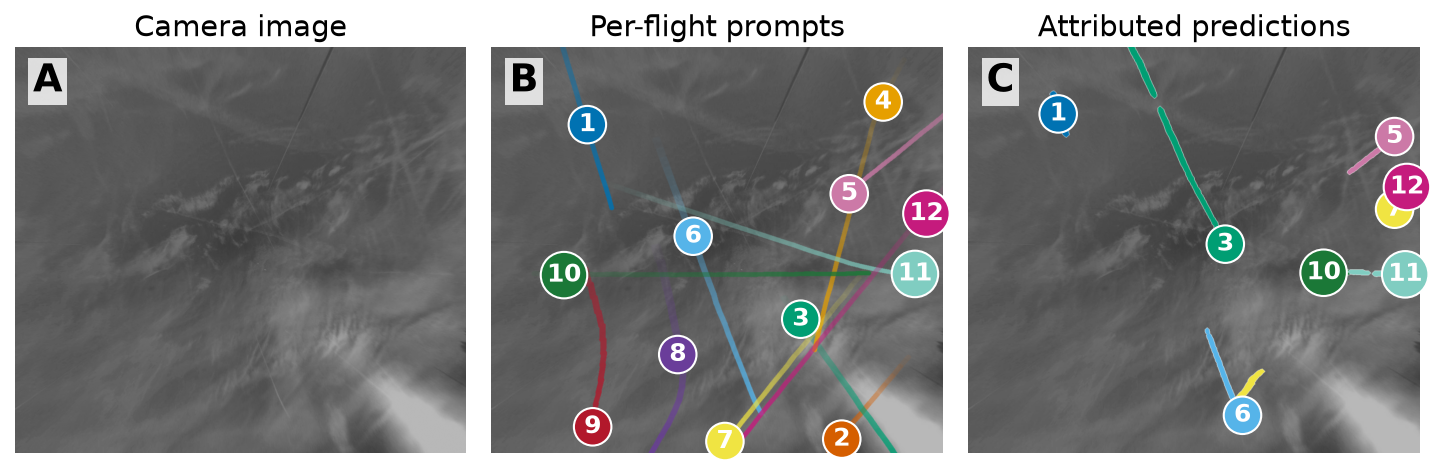
\includegraphics[width=\linewidth]{figures/fig_attribution_scene.png}
\caption{Attribution in action (video~2, frame~176, age-weighted with negative signal, 5-min variant). (A)~Raw camera image with multiple simultaneous contrails. (B)~Per-flight positive age-weighted prompts: each numbered color corresponds to one flight's predicted contrail polygon (negative suppression signals are not shown for clarity). (C)~Predictions in matching colors and numbers. Identity is established by construction: no post-hoc matching step is needed. Of the 12 prompted flights, 8 are confirmed with segmentation masks; flights 2, 4, 8, and~9 produce no prediction (prompt rejection), shown by the absence of their number in panel~C.}
\label{fig:attribution_scene}
\end{figure}

\subsection{Prompt Design Comparison}

Table~\ref{tab:ablation} presents the results for all five variants.

\begin{table}[!tbp]
\centering
\caption{Prompt design comparison on the GVCCS test set (610 flights with ground truth, 2{,}822 negative-example flights). All variants use the same SAM2.1 Hiera~B+ architecture. The four age-weighted variants form a 2$\times$2 grid: negative signal (absent vs.\ present) $\times$ age window (5 vs.\ 10~min). Binary uses a flat 1-min mask without age weighting; its row therefore conflates encoding and window (Section~\ref{sec:results}). Training epochs are tuned per variant based on convergence analysis (Section~\ref{sec:training}). \textbf{Bold} marks the best value in each column; ties are bolded jointly. Precision and Wrong-attribution rate are computed over matched predictions (IoU~$\geq$~0.25) across all frames; Recall is first-detection attribution over all GT flights and equals Detection~$\times$~first-frame precision. Video-level bootstrap 95\% confidence intervals for the headline metrics are shown in Fig.~\ref{fig:metrics_ci}.}
\label{tab:ablation}
\resizebox{\linewidth}{!}{%
\begin{tabular}{l l c c c c c c c c c}
\toprule
& & \multicolumn{3}{c}{\textbf{Segmentation}} & \multicolumn{3}{c}{\textbf{Tracking}} & \multicolumn{3}{c}{\textbf{Attribution}} \\
\cmidrule(lr){3-5} \cmidrule(lr){6-8} \cmidrule(lr){9-11}
\textbf{Encoding} & \textbf{Window} & mAP$_{25{:}75}$ & mAP$_{25}$ & mAP$_{75}$ & Detection & Completeness & Temp. IoU & Precision & Recall & Wrong \\
\midrule
Binary (flat)           & 1 min  & 0.303 & 0.579 & 0.024 & \textbf{93.4\%} & 0.724 & 0.500 & 89.0\% & 87.2\% & 11.0\% \\
\midrule
\multirow{2}{*}{Age-weighted} & 5 min  & 0.369 & 0.666 & \textbf{0.034} & 91.3\% & 0.709 & 0.510 & 96.1\% & 88.5\% & 3.9\% \\
                               & 10 min & 0.348 & 0.629 & 0.033 & 87.9\% & 0.642 & 0.489 & \textbf{96.4\%} & 84.6\% & \textbf{3.6\%} \\
\midrule
\multirow{2}{*}{\shortstack[l]{Age-wtd.\ +\\neg.\ signal}} & 5 min  & \textbf{0.380} & \textbf{0.693} & \textbf{0.034} & 92.6\% & \textbf{0.730} & \textbf{0.516} & 96.2\% & \textbf{90.3\%} & 3.8\% \\
                         & 10 min & 0.364 & 0.657 & 0.033 & 90.0\% & 0.688 & 0.501 & \textbf{96.4\%} & 87.2\% & \textbf{3.6\%} \\
\bottomrule
\end{tabular}}
\end{table}

\paragraph{Both design axes act independently.} One caveat applies to the comparison with binary: the binary baseline uses a 1-min window while the age-weighted variants use 5 or 10~min, so encoding richness and window width are conflated in that row. Within the 2$\times$2 grid, the window axis is isolated by comparing 5-min and 10-min within each encoding block, and the encoding axis is isolated by comparing age-weighted and negative-signal within each window block. Age-weighted prompts raise mAP$_{25{:}75}$ from 0.303 (binary) to 0.369 at 5~min (+21.8\%) and 0.348 at 10~min (+14.9\%): temporal context in the encoding benefits segmentation at both window sizes. Adding the negative signal pushes further---0.380 at 5~min (+3.0\% over age-weighted) and 0.364 at 10~min (+4.6\%). The best variant improves mAP$_{25{:}75}$ by 25.4\% relative to binary. Shortening the window from 10 to 5~min also helps at both encoding levels: +6.0\% for age-weighted, +4.4\% with the negative signal. These gains are roughly additive across the grid---the two axes are close to independent. The pattern holds at every IoU threshold (Fig.~\ref{fig:ap_curves}): the absolute separation between the best variant and binary is largest ($0.11$--$0.12$~AP) at permissive thresholds (0.25--0.40) and narrows toward the strict end, while the \emph{relative} improvement grows with the threshold. At the strict end, all non-binary variants lift mAP$_{75}$ from 0.024 to 0.033--0.034: richer prompts sharpen boundaries, not just coverage.

\begin{figure}[!tbp]
\centering
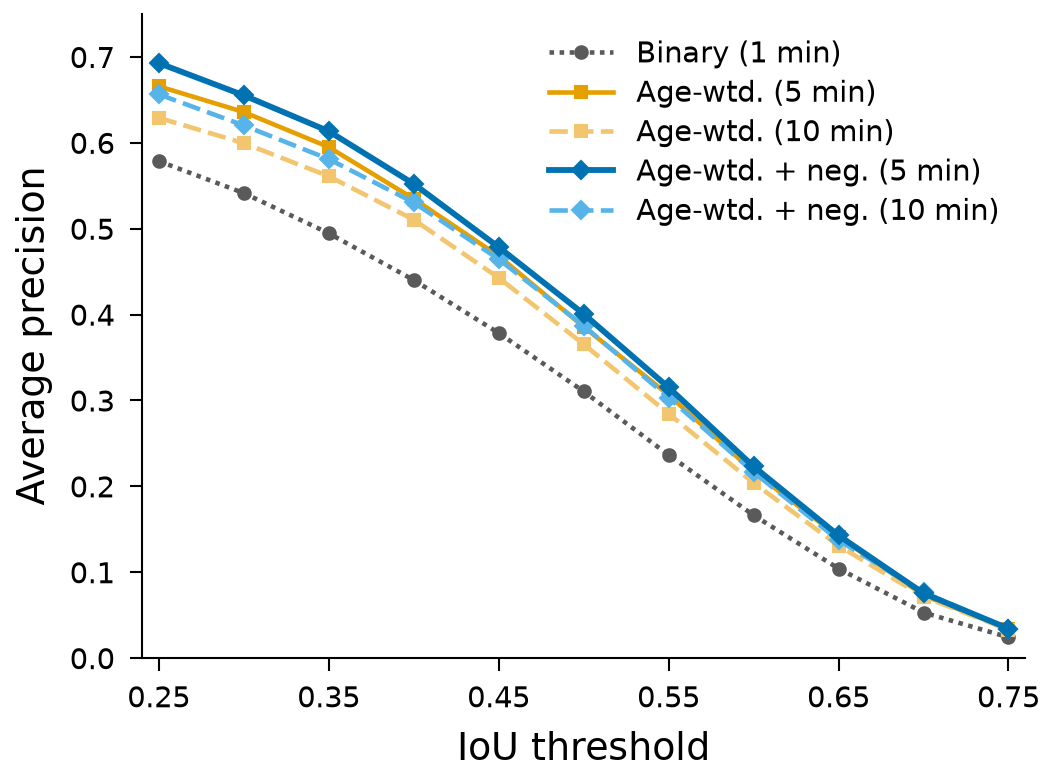
\includegraphics[width=3.5in]{figures/fig_ablation_ap_curves.png}
\caption{Average precision at each IoU threshold for all five variants. Color encodes the prompt family (gray: binary; orange: age-weighted; blue: age-weighted with negative signal); solid lines mark 5-minute windows and dashed lines 10-minute windows. Adding the age gradient and the negative signal shifts the whole curve upward; the absolute gap over binary is largest at permissive thresholds, while the relative gain grows toward the strict end.}
\label{fig:ap_curves}
\end{figure}

\paragraph{The 5-minute window resolves the detection--quality tradeoff.} The 10-minute variants pay a detection-rate penalty: 87.9\% (age-weighted) and 90.0\% (with negative signal) versus 93.4\% for binary. The cause is prompt drift---10-minute-old geometry has accumulated enough ERA5 wind error that the prompt no longer sits on the contrail, and the model treats the mismatch as evidence that no contrail is present. The 5-minute variants recover most of this loss: 91.3\% (age-weighted) and 92.6\% (with negative signal). Five minutes is short enough that ERA5 errors stay within the model's spatial tolerance, yet long enough for the age gradient and negative signal to improve boundary quality. Track completeness tells the same story: 0.730 with the negative signal at 5~min, versus 0.688 at 10~min, 0.709 for age-weighted 5~min, and 0.724 for binary.

\paragraph{Attribution.} All non-binary variants reach attribution precision above 96\%, a substantial jump from 89.0\% for binary. This 7-point gap is the single largest effect of adding temporal structure to prompts: without the age gradient, the model confuses overlapping flights at a much higher rate (11.0\% wrong attributions for binary versus 3.6--3.9\% for all other variants). The gain is flat across non-binary variants (96.1--96.4\%) regardless of whether the negative signal is present or which window is used, suggesting that the age gradient alone accounts for most of the improvement. Attribution recall rises from 87.2\% (binary) to 88.5\% (age-weighted 5~min) to 90.3\% (with negative signal, 5~min). Section~\ref{sec:discussion} explains the mechanisms behind both effects.

\paragraph{Identity quality.} Table~\ref{tab:identity} extends two identity-centric metrics---fragmentation and cross-contamination---to all five variants (the original submission reported them only for the best variant). Binary tracking is markedly worse on both: its mean fragmentation of 1.19 indicates that roughly one in five contrails is split across multiple prediction identities, whereas every age-weighted variant stays at or near 1.0, and 17.6\% of binary's overlap events are high-contamination (mask overlap ratio above 50\%) against 6.5--8.0\% for the richer encodings. Both failure modes---identity splits and pixel leakage across flights---are precisely the errors that corrupt attribution in sequential pipelines, and both are largely eliminated by the age gradient, with the negative signal providing a further reduction in high-contamination events at each window size.

\begin{table}[!tbp]
\centering
\caption{Identity quality across all five variants. Fragmentation is the mean number of prediction identities covering each ground truth contrail (1.0 = one identity per contrail; flights never detected contribute 0). Contamination events count (prediction, frame) pairs whose mask overlaps another flight's ground truth; high events are those with overlap ratio $>$50\%.}
\label{tab:identity}
\begin{tabular}{l l c c c}
\toprule
\textbf{Encoding} & \textbf{Window} & \textbf{Fragm.} & \textbf{Contam. events} & \textbf{High ($>$50\%)} \\
\midrule
Binary (flat) & 1 min & 1.19 & 13{,}614 & 2{,}402 (17.6\%) \\
\midrule
\multirow{2}{*}{Age-weighted} & 5 min & 1.00 & 8{,}560 & 687 (8.0\%) \\
 & 10 min & 0.96 & 8{,}227 & 613 (7.5\%) \\
\midrule
\multirow{2}{*}{\shortstack[l]{Age-wtd.\ +\\neg.\ signal}} & 5 min & 1.01 & 8{,}672 & 641 (7.4\%) \\
 & 10 min & 0.98 & 8{,}726 & 566 (6.5\%) \\
\bottomrule
\end{tabular}
\end{table}

\subsection{How Much Does the Visual Model Add? A Prompt-as-Prediction Baseline}
\label{sec:promptbaseline}

Because prompts already encode where physics expects each contrail, one may ask how much of the reported accuracy is contributed by SAM2 at all. We therefore evaluate a training-free baseline that treats the rasterized CoCiP prompt itself (binarized, 5-minute window) as the predicted mask on every ground truth frame. The physics prior alone is far from a usable segmentation: across the 14{,}262 ground truth frames of the 610 annotated flights, the raw prompt achieves a mean IoU of 0.042 against the annotation (median 0.0), reaches IoU~$\geq$~0.25 on only 4.6\% of frames, and only 0.8\% of flights attain a mean IoU above 0.25. Three factors drive this gap: wind-advection error displaces the prompt from the visible contrail, the projected polygon is systematically wider or narrower than the observed plume, and prompts persist on frames where the contrail is not (or not yet) visible. The trained model lifts mean temporal IoU from 0.042 to 0.516 and frame-level matching from 4.6\% to 73\% (completeness)---the visual refinement, not the physics prior, contributes essentially all of the segmentation accuracy, while the prior contributes the localization and the identity.

\subsection{Uncertainty Quantification}
\label{sec:uncertainty}

All metrics in Table~\ref{tab:ablation} are point estimates on a single test set; to assess their stability we compute cluster bootstrap confidence intervals that respect the correlation structure of the data: entire videos (the 18 test sequences containing annotated flights) are resampled with replacement 10{,}000 times, and every per-flight or per-prediction record from a sampled video enters the pooled statistic. Fig.~\ref{fig:metrics_ci} shows the resulting 95\% intervals for the four headline metrics.

\begin{figure}[!tbp]
\centering
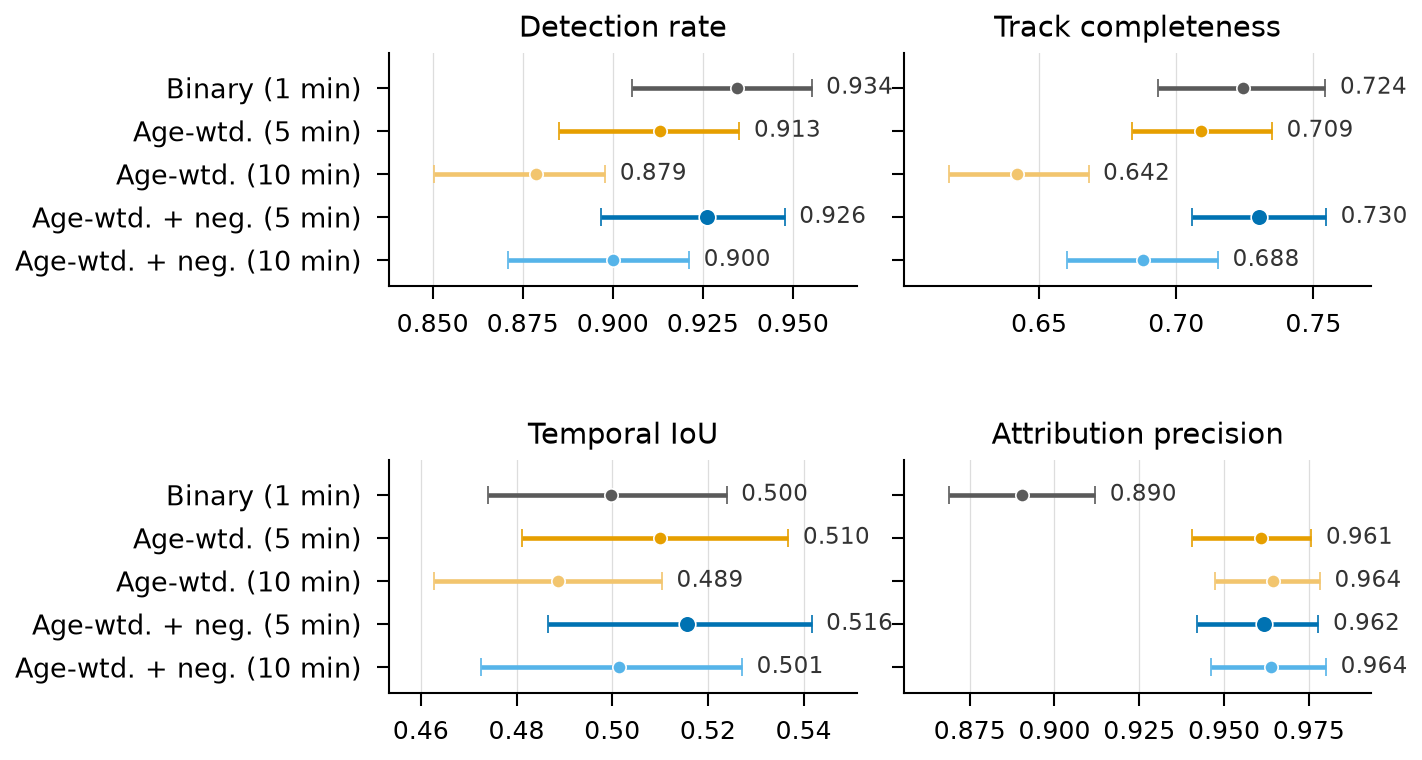
\includegraphics[width=\linewidth]{figures/fig_metrics_ci.png}
\caption{Headline metrics with 95\% video-level bootstrap confidence intervals (10{,}000 resamples of the 18 annotated test videos). Color encodes the prompt family (gray: binary; orange: age-weighted; blue: age-weighted with negative signal); saturated marks denote 5-minute windows. The attribution-precision panel isolates the paper's central effect: binary sits 7 points below every age-weighted variant with non-overlapping intervals, while the detection-rate and completeness differences between binary and the best variant lie within resampling noise.}
\label{fig:metrics_ci}
\end{figure}

Fig.~\ref{fig:completeness_dist} complements the interval estimates with the underlying per-flight distributions. The survival curves show that the best variant keeps more flights above every completeness level up to roughly 0.8, beyond which the binary baseline briefly leads, and the paired panel explains why the mean difference is small: most flights are tracked equally well by both variants (330 of 610 within $\pm$0.02), while 133 flights improve and 147 regress, with large movements in both directions. The aggregate near-tie in completeness therefore reflects offsetting redistribution rather than the absence of an effect.

\begin{figure}[!tbp]
\centering
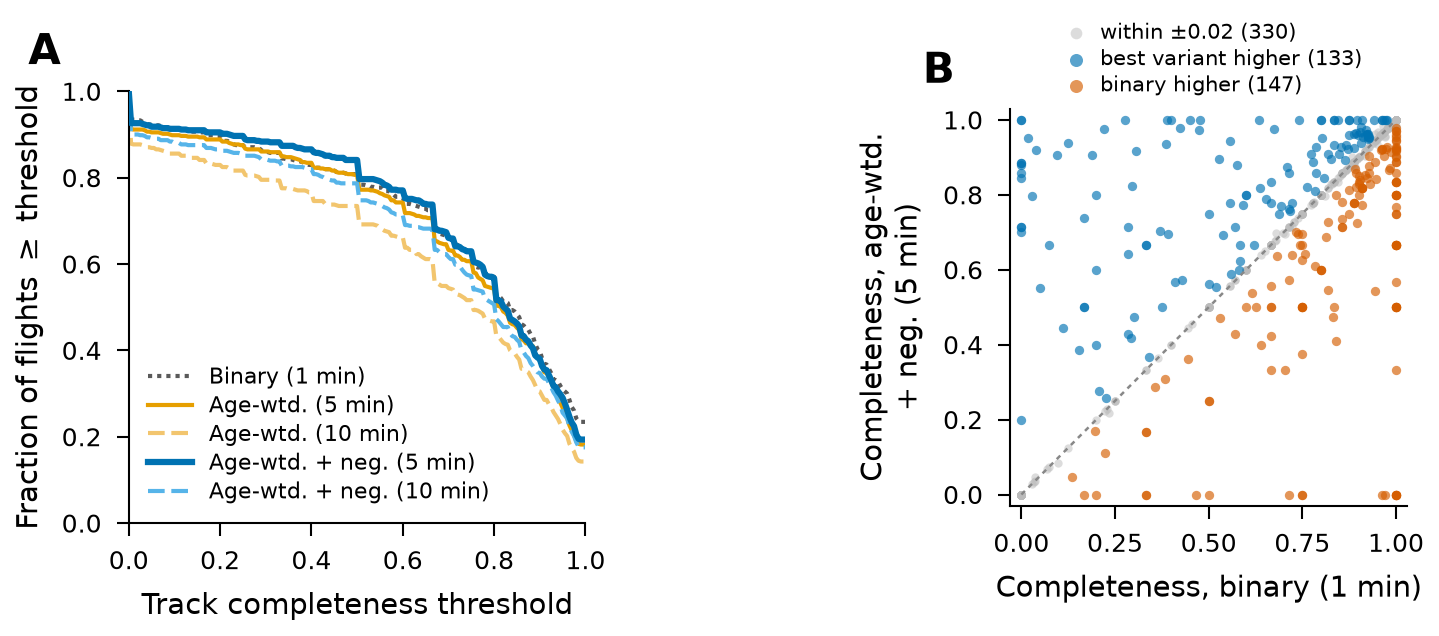
\includegraphics[width=\linewidth]{figures/fig_completeness_dist.png}
\caption{Per-flight track completeness. (A)~Fraction of the 610 annotated flights whose completeness meets each threshold, for all five variants (color: prompt family; solid: 5-min window; dashed: 10-min window; dotted: binary). (B)~Paired per-flight comparison of the binary baseline and the best variant; each point is one flight, and counts give flights above, on, and below the diagonal (a $\pm$0.02 band counts as a tie).}
\label{fig:completeness_dist}
\end{figure}

Three conclusions follow. First, the attribution-precision gap between binary and every age-weighted variant is decisively significant: the paired video-level bootstrap for the best variant minus binary gives $+7.1$ points with 95\% CI $[+5.4, +8.9]$ and $p(\Delta \le 0) < 10^{-4}$, and the same holds for temporal IoU ($+0.016$, CI $[+0.008, +0.024]$). Second, the within-grid effects are also robust: at the 5-minute window, adding the negative signal significantly improves completeness ($+0.021$, CI $[+0.011, +0.030]$) and detection rate ($+0.013$, CI $[+0.005, +0.020]$); at fixed age-weighted encoding, shortening the window from 10 to 5 minutes significantly improves completeness ($+0.067$), detection rate ($+0.035$), and temporal IoU ($+0.021$), all with $p(\Delta \le 0) < 10^{-2}$. Third, the differences in detection rate ($-0.8$ points, CI $[-2.2, +0.8]$) and completeness ($+0.6$ points, CI $[-1.2, +2.5]$) between the binary baseline and the best variant are \emph{not} statistically distinguishable: the binary baseline finds contrails about as often as the best variant---what it cannot do is delineate them as accurately or attribute them as reliably. We therefore claim the segmentation-quality and attribution gains as the robust contributions of richer prompts, not raw detection coverage.

\subsection{Visual Analysis}

\paragraph{Tracking sequence.} Fig.~\ref{fig:tracking_sequence} shows four frames sampled from a 25-frame tracking window (frames 205--229) in which the best variant (age-weighted with negative signal, 5~min) follows flight 34ba902a (video~14) through a scene dense with competing traffic. Under the binary baseline this flight reaches 40.9\% completeness; the age-weighted with negative signal variant raises it to 56.8\%. The prompt row makes the difficulty of the scene immediately visible: magenta regions indicate where competing contrails from other flights claim the image, while a narrow blue band marks the target contrail's predicted position. The negative signal suppresses attention to competing structures and allows SAM2 to lock onto the correct trajectory, with prediction scores rising from 0.76 to 0.94 across the shown frames as the visual evidence accumulates in memory.

\begin{figure}[!tbp]
\centering
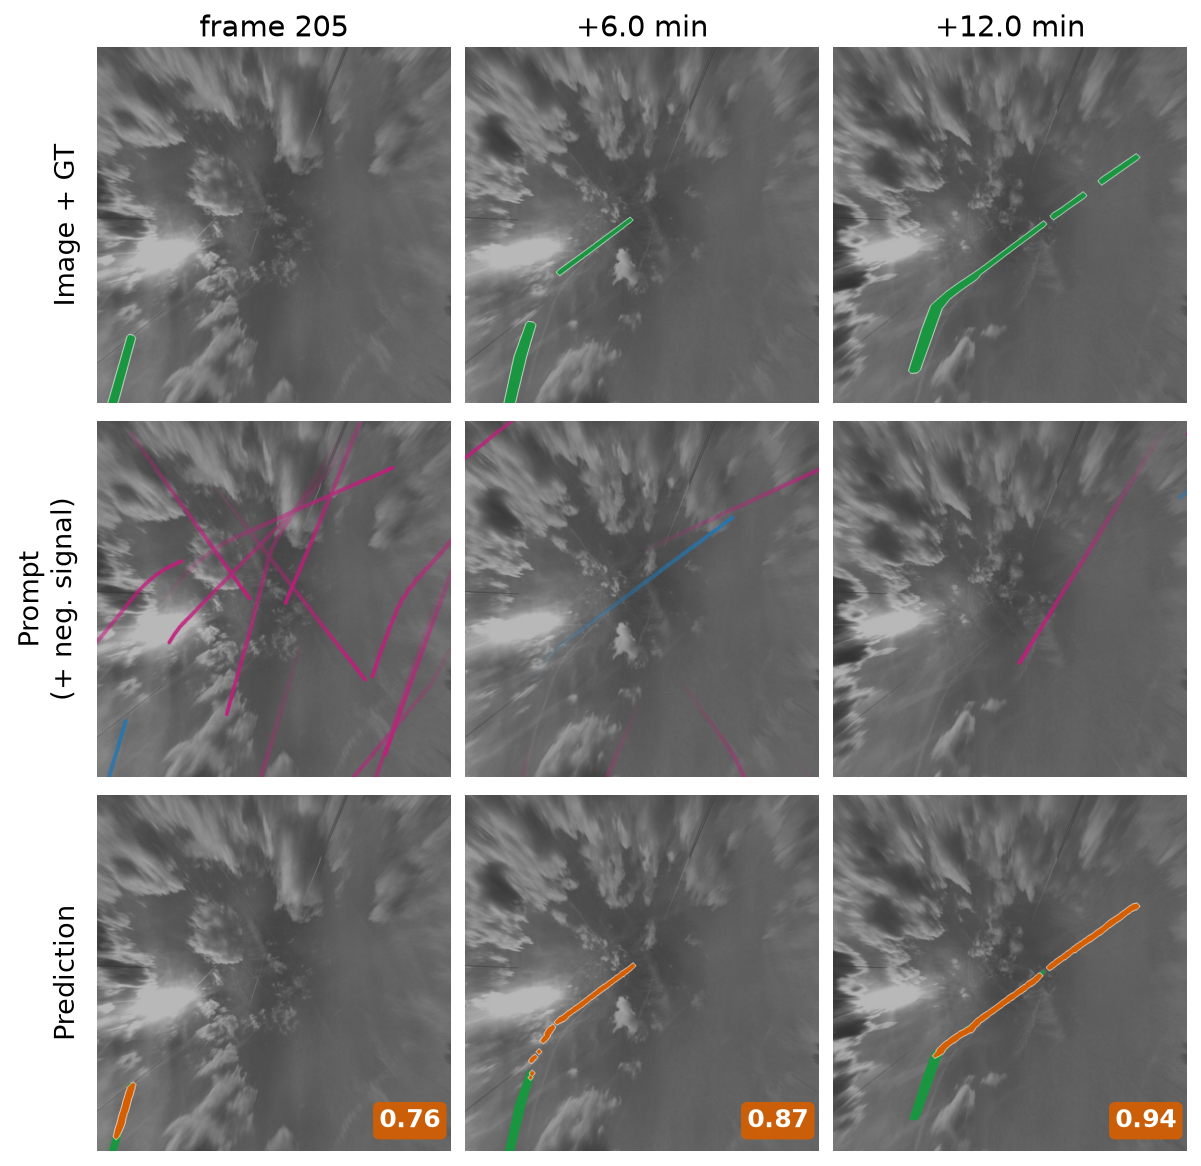
\includegraphics[width=\linewidth]{figures/fig_examples.png}
\caption{Tracking sequence for flight 34ba902a (video~14, age-weighted with negative signal, 5-min variant); columns are frames 205--229, labelled by elapsed time at the 30-second GVCCS cadence. Row~1: image with ground truth overlay (green). Row~2: age-weighted prompt with negative signal overlay---\textit{blue} marks the target flight's age-weighted footprint; \textit{magenta} marks regions attributed to competing flights (the negative suppression signal). Row~3: prediction overlay (vermilion) with object score badge; the solid green underlay repeats the ground truth for comparison. On this flight the variant reaches 56.8\% completeness (vs.\ 40.9\% for the binary baseline), with scores rising from 0.76 to 0.94 across the shown frames.}
\label{fig:tracking_sequence}
\end{figure}

\paragraph{Both design axes on a single flight.} Fig.~\ref{fig:variant_comparison} shows all five variants on flight 324b5d6a (video~12), whose per-variant track completeness spans nearly the full range observed in the aggregate ablation: 31\% for binary, 89\% for age-weighted 5-min, 92\% with the negative signal at 5~min, but only 39\% and 33\% for the two 10-minute variants. Every variant produces scored predictions on most frames---the score badges in the figure are consistently above the 0.5 threshold---so the differences are not about finding the contrail but about delineating it: the binary and 10-minute predictions sit displaced from the annotated contrail and fail the IoU~$\geq$~0.25 match, while the 5-minute age-weighted prompts keep the prediction locked onto the visible contrail across its lifetime. The example illustrates, on one flight, the two aggregate effects that the paired bootstrap confirms across the test set (Section~\ref{sec:uncertainty}): the age gradient at a short window drives match quality, and widening the window to 10~minutes lets accumulated wind drift pull the prompt---and with it the prediction---off the contrail.

\begin{figure}[!tbp]
\centering
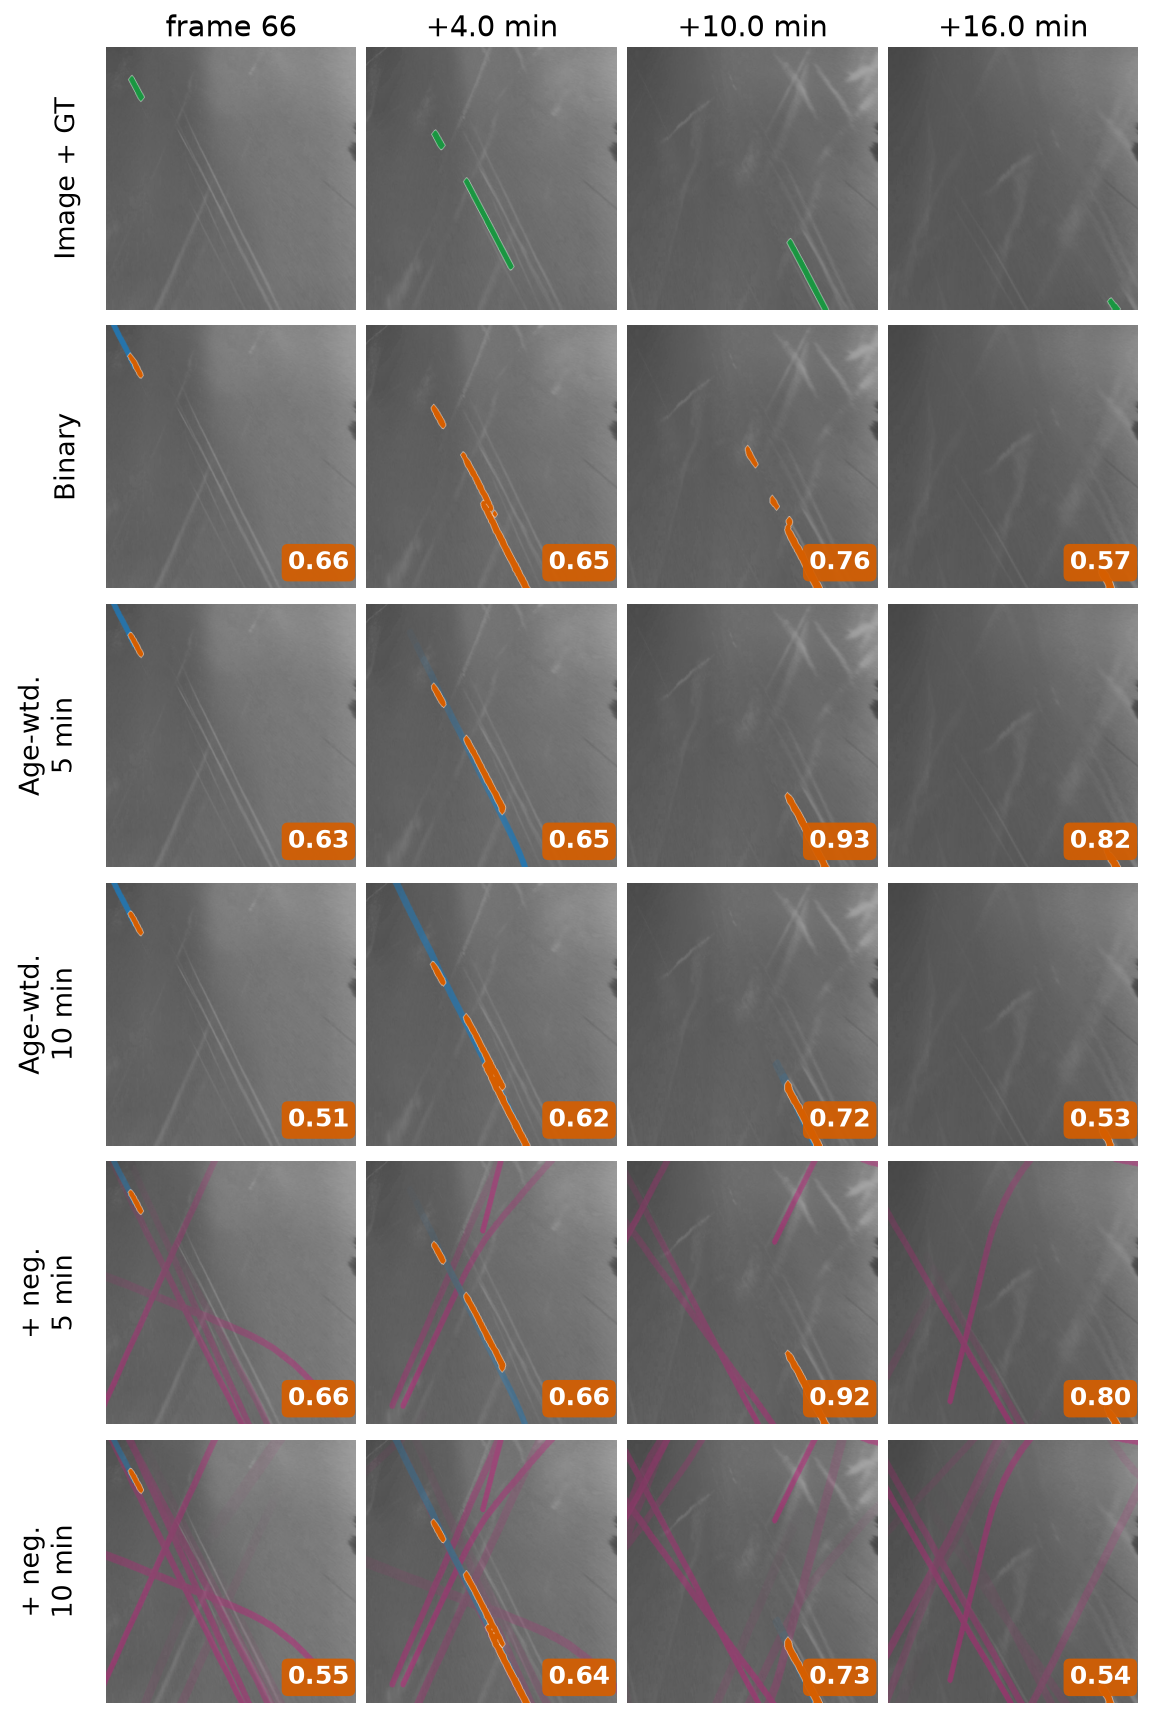
\includegraphics[width=\linewidth]{figures/fig_variant_comparison.png}
\caption{Flight 324b5d6a (video~12) tracked by all five variants; columns are labelled by elapsed time (30-second cadence). Row~1: image with ground truth overlay (green, thickened for visibility). Rows~2--6: per-variant prompt and prediction---flat \textit{blue} for the binary prompt, \textit{blue} gradient for age-weighted prompts, plus \textit{magenta} competing-flight suppression for the negative-signal variants; vermilion shows the predicted mask (thickened for visibility) with its object-score badge. All variants fire confidently on most frames, but only the 5-minute age-weighted variants keep the mask on the annotated contrail (completeness 89\% without and 92\% with the negative signal, vs.\ 31\% for binary and 39\%/33\% for the drift-affected 10-minute variants).}
\label{fig:variant_comparison}
\end{figure}

\paragraph{Age window trade-off.} The choice of age window interacts with scene density in ways that headline metrics do not capture. Fig.~\ref{fig:window_comparison} shows two contrasting cases. Case~A (flight 3363798b, video~5) shows a contrail that is already several minutes old when it becomes clearly visible: the 5-minute window covers only the recent tip, giving the model too small a footprint to confirm detection (2.7\% completeness), while the 10-minute window extends the prompt back along the full visible contrail and achieves 70.3\% completeness. Case~B (flight 33c16444, video~7) is the mirror situation: multiple older contrails cross the scene, and the 10-minute window picks them up as negative signal. The resulting suppression is too aggressive, reducing completeness to 0\%. The 5-minute window avoids this contamination and achieves 100\% completeness, with SAM2's memory continuing to track the contrail after the prompts end. These two cases suggest that the optimal window depends on per-flight geometry and surrounding traffic density---an adaptive window calibrated to ERA5 wind uncertainty and local scene density is a natural extension of this work.

\begin{figure}[!tbp]
\centering
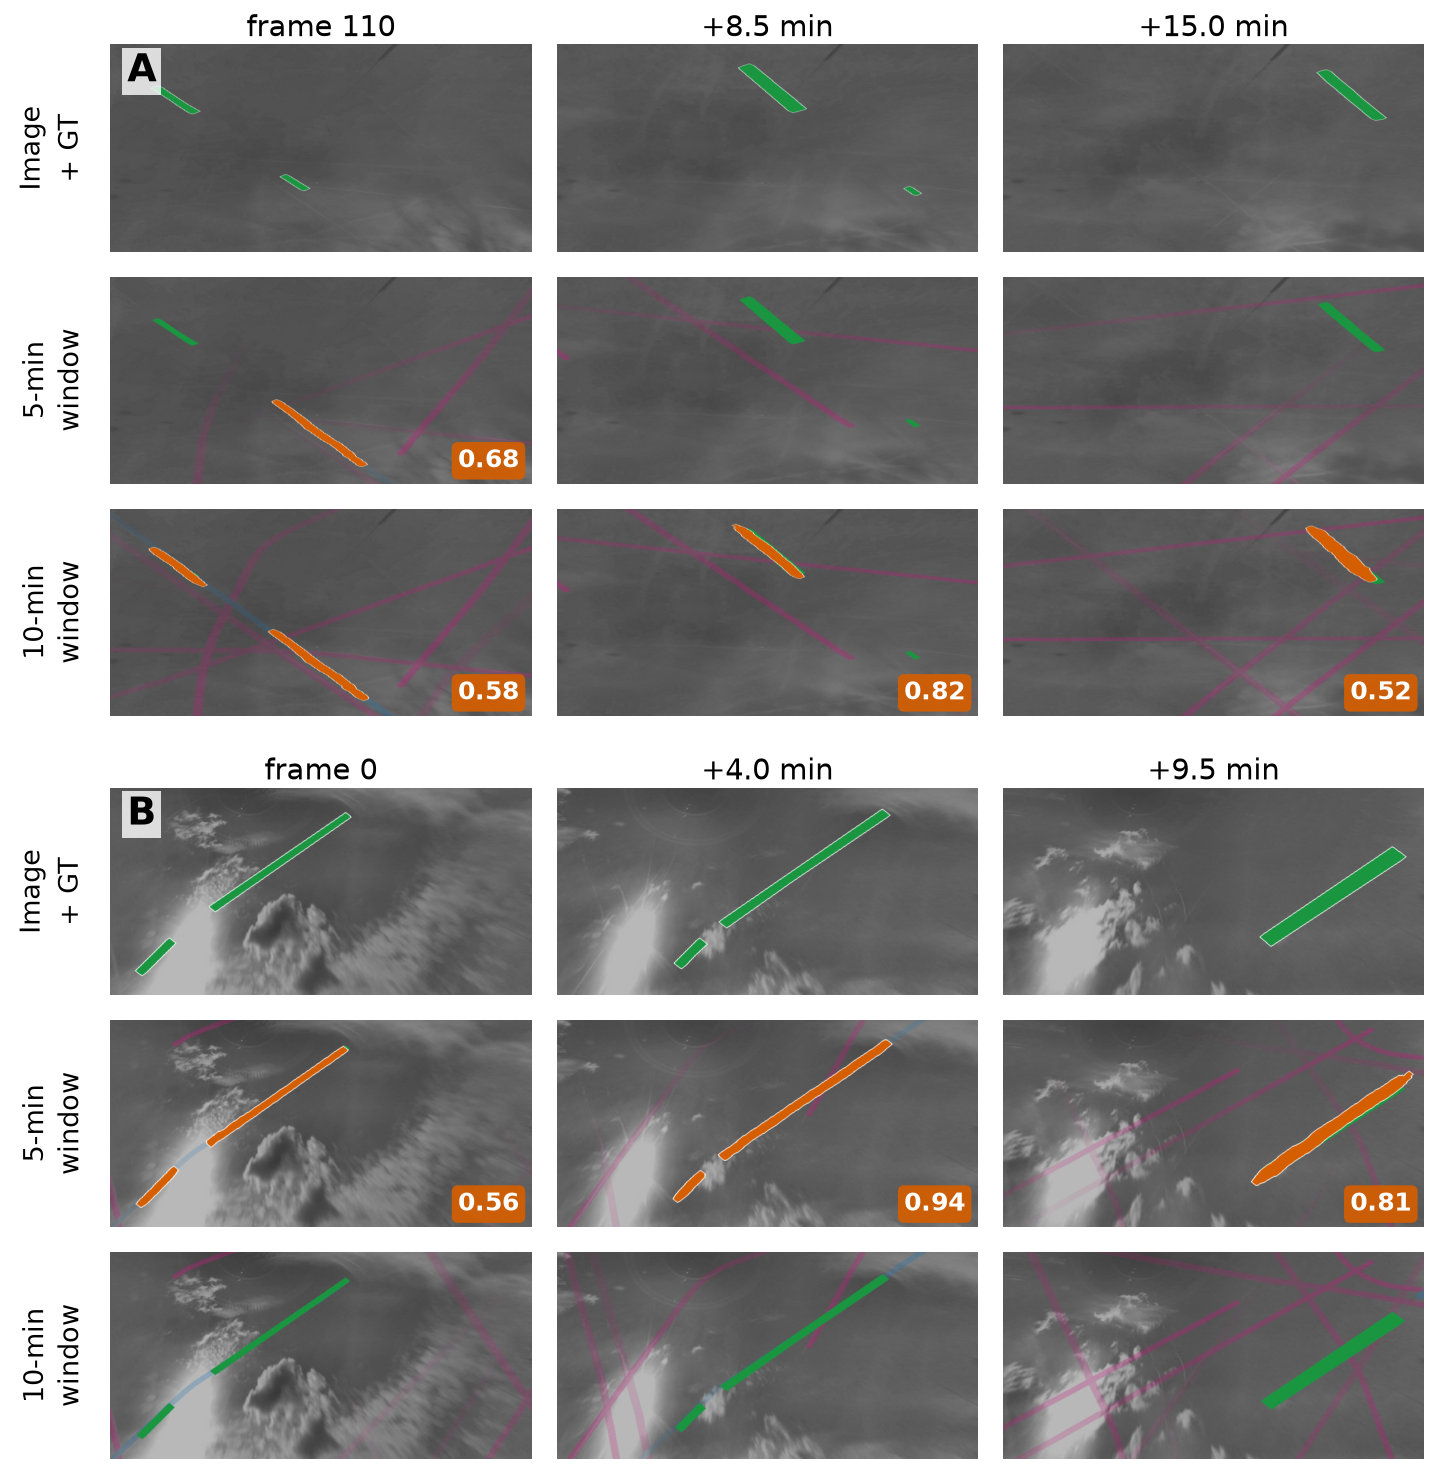
\includegraphics[width=\linewidth]{figures/fig_window_comparison.png}
\caption{Age-window trade-off on two contrail flights, both tracked by the age-weighted with negative signal encoding; columns are labelled by elapsed time (30-second frame cadence). Row~1 of each case: image with ground truth overlay (green, thickened for visibility). Rows~2--3: 5- and 10-minute windows---\textit{blue} tint shows the target flight's age-weighted prompt, \textit{magenta} tint the suppression signal from competing flights, vermilion the predicted mask with its object-score badge, and a solid green underlay repeats the ground truth. Case~A (flight 3363798b, video~5): the contrail becomes clearly visible only minutes after formation; the 5-min window covers too small a footprint---its two scored predictions fail the IoU~$\geq$~0.25 match against ground truth---while the 10-min window extends the prompt along the full contrail (2.7\% vs.\ 70.3\% completeness). Case~B (flight 33c16444, video~7): older unprompted contrails cross the scene; under the 10-min window they enter the negative signal and suppress the true detection (0\% completeness), whereas the 5-min window avoids the contamination (100\%).}
\label{fig:window_comparison}
\end{figure}

\subsection{Prompt Discrimination}
\label{sec:discrimination}

Most prompted flights do not produce visible contrails in the GVCCS dataset, so the model must learn to say ``no.'' We evaluate this through the object score, a scalar output indicating confidence that a contrail is present. For each prompted flight we take the maximum score over its video; a flight whose prompts never trigger any prediction receives a score of zero. Under the 5-minute window, 2{,}609 of the 3{,}432 prompted flight--video pairs produce at least one non-empty prompt raster; 610 of these have ground truth annotations (visible contrails) and 1{,}999 do not.

Fig.~\ref{fig:discrimination} shows the resulting score distributions and the receiver operating characteristic (ROC) of prompt rejection for the best variant. The inference pipeline records predictions only above its 0.5 decision threshold, so flights that never cross it appear at score zero; rates at the 0.5 operating point are therefore exact, while the AUC treats sub-threshold flights as ties. The two populations are well separated: flights with a visible contrail reach a mean maximum score of 0.79, against 0.04 for empty prompts, and the area under the ROC curve is 0.97 (video-level bootstrap 95\% CI $[0.94, 0.97]$). At the operational threshold of 0.5, the model confirms 94.3\% of flights with visible contrails (5.7\% false-negative rate) while rejecting 93.5\% of empty prompts (6.5\% false-positive rate). Because 76\% of prompts in the test set are negatives, this operating point matters: a model that blindly trusted its prompts would triple the number of reported contrails. The residual errors are faint contrails the model misses and coincidental contrail-like features under empty prompts; the failure-mode analysis below quantifies both.

\begin{figure}[!tbp]
\centering
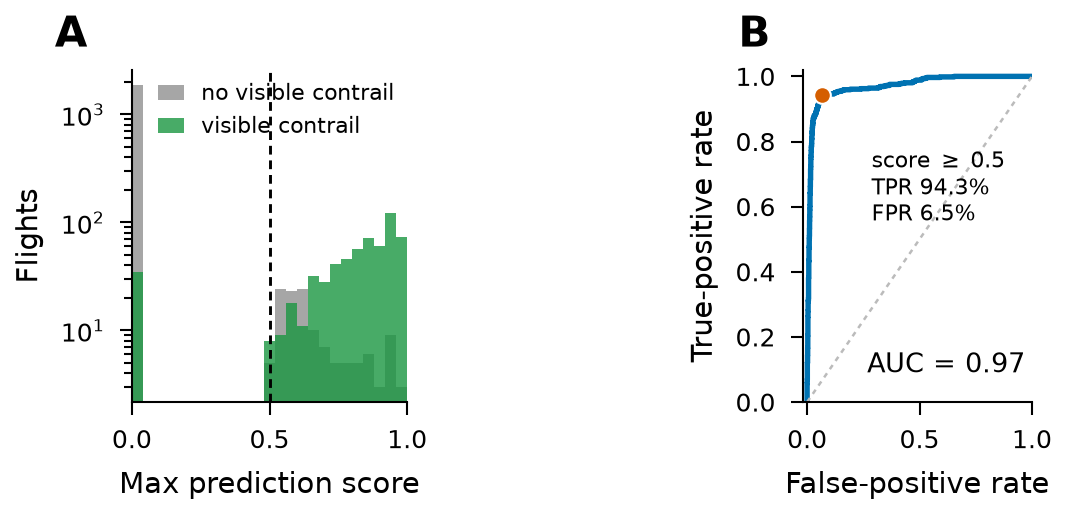
\includegraphics[width=\linewidth]{figures/fig_discrimination.png}
\caption{Prompt rejection by the best variant (age-weighted with negative signal, 5~min). (A)~Distribution of per-flight maximum prediction scores (log-scale counts): flights with a visible (annotated) contrail in green, prompted flights without a visible contrail in gray; the dashed line marks the operational 0.5 threshold. (B)~ROC curve of accepting a flight based on its maximum score (AUC~0.97); the marker shows the 0.5 operating point (true-positive rate 94.3\%, false-positive rate 6.5\%).}
\label{fig:discrimination}
\end{figure}

\subsection{Training Convergence}
\label{sec:training}

Age-weighted variants reach lower total loss ($\sim$4.0) than binary ($\sim$5.3) at comparable epochs. The richer continuous signal gives the model more to work with per frame, and the loss curve flattens accordingly. Binary prompts converge more slowly because the model must recover temporal context from visual features alone.

How long to train depends on the prompt. The 10-minute variants produce denser prompt masks, and their loss curves decrease smoothly through 20~epochs with no sign of saturation. The 5-minute variants plateau around epoch~10 and fluctuate afterward---the effective training signal per sample is smaller, and the model starts fitting noise. Binary prompts overfit hardest: training loss keeps falling past epoch~10, but test-set segmentation gets worse. We confirmed this directly: the 20-epoch binary checkpoint produced visibly degraded masks compared to the 10-epoch checkpoint on the same test videos.

We therefore train each variant for a different number of epochs: 10 for binary, 15 for the 5-minute variants, 20 for the 10-minute variants. This per-variant tuning is a confound: the richer variants receive more training iterations, so part of their advantage could stem from longer training rather than prompt design alone. We selected epochs from training loss curves rather than test-set metrics, but the binary overfitting was confirmed on test videos, which constitutes a form of test-set selection (see Section~\ref{sec:dataset} for the no-validation-set rationale). A fully controlled comparison would evaluate all variants at a single common epoch count; we did not conduct this experiment, and acknowledge it as a limitation. The direction of the confound, however, is conservative for the richer variants: binary reaches its best performance at 10 epochs and degrades thereafter, while age-weighted variants continue improving through 15--20 epochs, so fixing epochs at 10 would likely widen, not narrow, the gap between binary and non-binary variants.

\subsection{Analysis of the Best Variant}

The previous subsections compared variants against each other. Here we examine the best-performing configuration (age-weighted with negative signal, 5~min) in more detail, focusing on what it does well and where it falls short.

\paragraph{Thin structures are hard.} The gap between mAP$_{25}$ (0.693) and mAP$_{75}$ (0.034) needs context. mAP$_{75}$ aggregates precision and recall over confidence thresholds at a strict IoU criterion; it is suppressed whenever high-confidence predictions cluster below the 0.75 boundary. The low value does not imply that nearly all contrails are missed---it reflects that accurate boundary delineation at IoU~$>$~0.75 is rare even when the contrail is detected and correctly located. The cause is geometric: at the memory encoder's $64\times64$ resolution, a contrail spanning 2~pixels in the original 1024$\times$1024 image occupies less than one memory pixel, and even small boundary errors at this scale substantially reduce IoU. Performance on medium-sized objects (mAP$_{25{:}75}$ = 0.521) is substantially higher than on small objects (0.371), confirming that the bottleneck is spatial resolution in the memory encoder, not the model's ability to recognize contrails.

\paragraph{Temporal consistency.} Fragmentation of 1.005 means each ground truth contrail is covered by essentially a single prediction identity (the small excess above 1.0 reflects rare frame-boundary effects where the last few frames of a fading contrail are picked up under a second short-lived prediction)---a direct consequence of the prompt-based architecture where each flight maintains its identity across all frames without appearance-based re-identification. In a conventional VOS pipeline, fragmentation would be higher because identity must be re-established at each frame through appearance matching, which fails when contrails change appearance (spreading, fading, changing brightness with sun angle). Our prompt-based identity is immune to these visual changes.

Track completeness of 0.730 means the model maintains detection, on average, across nearly three-quarters of a contrail's visible lifetime. Detection is also prompt: among flights the best variant ever attributes correctly, the median delay between a contrail's first annotated frame and its first correct detection is zero frames, the 90th percentile is one minute, and 96.6\% are confirmed within two minutes of first visibility---relevant for the envisaged monitoring application, where feedback about an avoidance maneuver is most useful while the aircraft is still in the sector. The remaining quarter corresponds to frames where model confidence drops below threshold, which occurs in three situations: (1)~the contrail becomes very faint, producing weak visual evidence; (2)~wind advection errors displace the prompt from the actual location by enough pixels that the model cannot find the contrail in the prompted region; or (3)~the contrail's appearance changes abruptly (e.g., sun angle changes) and the model briefly loses confidence before recovering from temporal memory.

\paragraph{Cross-contamination.} When multiple flights have nearby prompts, the model may segment one flight's contrail under another flight's prompt. Table~\ref{tab:identity} shows that the age gradient cuts high-contamination events by more than half relative to binary, and the negative signal reduces them further at each window (7.4\% of 8{,}672 events for the 5-min negative-signal variant). The remaining contamination is partly a data artifact: in dense airspace, ground truth masks from different flights naturally overlap because contrails spread and merge over time.

\subsection{Failure Modes}

We manually categorized the 50 lowest-performing flights (by temporal IoU) from the best variant to understand where the system fails. Fig.~\ref{fig:failure_modes} illustrates the three dominant modes on real test frames.

\begin{figure}[!tbp]
\centering
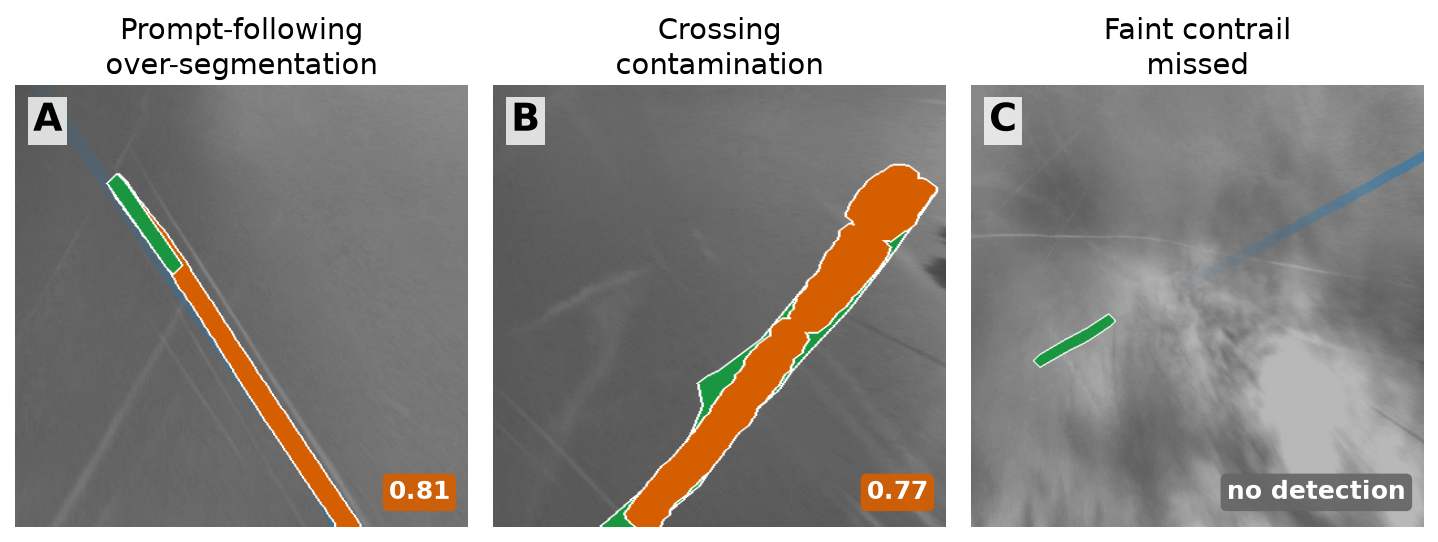
\includegraphics[width=\linewidth]{figures/fig_failure_modes.png}
\caption{Three characteristic failure modes of the best variant (ground truth in green, prompt in blue/magenta, prediction in vermilion; masks thickened for visibility). (A)~Prompt-following over-segmentation (flight 324b62ce, video~12): the wind-drifted prompt no longer matches the short visible contrail, and the model traces the prompt; the confident mask (score 0.81) covers the annotation but is far larger, so it fails the IoU match. (B)~Crossing contamination (video~12, frame~97): flight 324b5124's prediction covers 86\% of neighbouring flight 324b65d8's annotated contrail. (C)~Faint contrail missed (flight 33638739, video~5): the contrail is annotated (green) but the model, prompted along the drifted blue band, never produces a detection.}
\label{fig:failure_modes}
\end{figure}

Wind estimation errors cause roughly one-third of failures. ERA5 wind fields miss mesoscale variability, and errors exceeding $\sim$5~m/s displace prompts by tens of pixels from the actual contrail. When displacement exceeds the model's spatial tolerance, the prompt provides misleading guidance and the model either rejects a real contrail (treating the mismatch as evidence of absence), or---as in Fig.~\ref{fig:failure_modes}A---traces the drifted prompt itself, producing a confident mask far larger than the visible contrail.

Overlapping prompts cause roughly one-quarter of errors, concentrated in busy airspace where many flights produce nearby contrails. When prompt masks overlap substantially, even the negative signal cannot fully disambiguate boundary pixels. It tells the model that another flight exists, but when two contrails are separated by only a few pixels, correct boundary assignment is beyond the model's spatial resolution.

Unprompted contrails account for about one-fifth of missed detections. These are real contrails that drifted into the field of view from regions without ADS-B coverage, or from flights too far away for reliable advection modeling. These are missed by design: the system only examines prompted locations, and cannot attribute what it cannot identify.

The remaining errors are discrimination failures: accepting empty prompts (false positives from coincidental visual features) or rejecting real contrails (false negatives on faint or partially occluded contrails where the visual evidence does not meet the model's confidence threshold).

% ============================================================================
\section{Discussion}
\label{sec:discussion}

Richer prompts and shorter age windows both help, and they do so for different reasons. This section traces the interaction between the two design axes and explains the attribution improvement.

\subsection{Window and Negative Signal Interact Weakly}

The numbers in Table~\ref{tab:ablation} are close to additive. Adding the negative signal gains $+0.016$ mAP$_{25{:}75}$ at 10~min ($0.364 - 0.348$) and $+0.011$ at 5~min ($0.380 - 0.369$). Shortening the window gains $+0.021$ for age-weighted ($0.369 - 0.348$) and $+0.016$ with the negative signal ($0.380 - 0.364$). Strict additivity predicts age-weighted 5-min at $0.348 + 0.016 = 0.364$; the actual 0.369 is slightly higher, pointing to mild synergy between spatial precision and the age gradient. But the dominant pattern is independence: both axes contribute at every point in the grid. The paired bootstrap of Section~\ref{sec:uncertainty} confirms that the corresponding within-grid effects on the tracking metrics are statistically robust rather than resampling noise.

The negative signal gains most at 5~minutes because prompt accuracy and competing-flight suppression reinforce each other. At 5~min, ERA5 wind errors have had less time to accumulate, so both the positive and negative signals are spatially reliable. At 10~min, older segments have drifted further from the actual contrail, partially undermining both signals. That age-weighted 5-min (mAP$_{25{:}75}$ 0.369) falls closer to negative-signal 5-min (0.380) than to age-weighted 10-min (0.348) confirms that prompt accuracy matters more than the negative signal alone.

The detection-rate pattern carries the most practical weight. Both 10-min variants fall significantly below binary (87.9\% and 90.0\% vs.\ 93.4\%); both 5-min variants close most of this gap (91.3\% and 92.6\%), to the point where the remaining deficit against binary is within resampling noise (Section~\ref{sec:uncertainty}). Five minutes is a sweet spot: wind errors remain within the model's spatial tolerance. Past 5~minutes, accumulated drift starts causing false rejections. Accurate prompts do not just sharpen boundaries---they restore detection reliability that wider windows sacrifice.

\subsection{Why Richer Prompts Improve Attribution}

Attribution precision jumps from 89.0\% (binary) to above 96\% for every non-binary variant---the single largest improvement from adding temporal structure to prompts. The binary model misattributes 11\% of predictions, mostly at flight crossings where flat masks provide no spatial cue for disambiguation. The age gradient reduces this to under 4\%: a bright prompt region (young, well-localized) is a stronger spatial cue than a dim one (old, drifted), even when two flights overlap in space. Most of this gain comes from the age gradient alone---age-weighted 5-min already reaches 96.1\%, and adding the negative signal raises it only to 96.2\%.

The negative signal matters for recall and contamination rather than precision. Attribution recall climbs from 87.2\% (binary) to 88.5\% (age-weighted 5-min) to 90.3\% (with negative signal, 5-min). The mechanism is straightforward: marking pixels as belonging to another flight suppresses missed detections at crossings. High-contamination events ($>$50\% overlap) drop accordingly, because the negative signal limits pixel leakage across flight boundaries.

\subsection{Computational Cost}

The system runs in three stages at inference. Prompt generation (flight advection and camera projection) runs on CPU and scales linearly with the number of active flights, taking approximately 0.3~s per frame for a typical scene of 10--20 active flights. SAM2 image encoding runs once per frame on GPU regardless of flight count ($\sim$0.15~s on an RTX~6000 Ada). Memory attention and mask decoding run once per prompted flight per frame ($\sim$5~ms per flight for decoding, plus per-object memory-bank updates). For a scene with 20 active flights, these components total well under one second per frame---more than an order of magnitude inside the 30-second inter-frame interval of the GVCCS camera. Because only the per-flight decoding scales with traffic, denser airspace (50+ flights) adds a fraction of a second and remains far within the inter-frame budget on current hardware.

\subsection{Future Directions}

Several extensions could improve the system. First, the prompt currently encodes only spatial location and age. SAM2's prompt encoder accepts arbitrary dense inputs, so additional channels could carry meteorological context that CoCiP already computes: the Schmidt-Appleman formation criterion (did thermodynamics predict a contrail here?), persistence probability, or even the local relative humidity over ice. These signals would let the model weight its confidence based on atmospheric conditions, not just geometry. Multi-channel prompts are a natural next step and require no architectural change---only wider prompt masks during training.

Second, adaptive age windows that tighten in calm conditions (small advection error, tight prompts) and widen in windy conditions (larger uncertainty, but more temporal context needed) could automate the detection--quality tradeoff without a fixed window choice. Third, the negative signal could be extended beyond binary ``other flight present / absent'' to encode distance and identity, telling the model not just that another flight is nearby but how close and how many. Fourth, combining prompt-based and detection-based approaches---using the prompting system for attributable contrails and a conventional detector for unprompted ones---would close the coverage gap for contrails from unknown or distant flights.

% ============================================================================
\section{Limitations}
\label{sec:limitations}

The main limitation is wind accuracy. ERA5 reanalysis fields have limited horizontal resolution and hourly temporal resolution, missing mesoscale variability, jet stream gradients, and turbulence. When wind errors exceed roughly 5~m/s, prompts can be displaced by tens of pixels from the actual contrail. Higher-resolution regional models or data assimilation that refines wind estimates from observed contrail motion could help.

Dense traffic is another limitation. When many flights pass through similar airspace, prompts overlap and the model struggles with boundary assignment even with the negative signal. This limitation is geometric: at some density of overlapping contrails, no prompt encoding can disambiguate which pixels belong to which flight without sub-pixel spatial precision.

Statistical uncertainty is quantified for the tracking and attribution metrics through the video-level bootstrap of Section~\ref{sec:uncertainty}, but not for mAP: resampling the mAP requires re-running the COCO evaluation inside every bootstrap replicate, which we leave to future work. The within-grid mAP differences (e.g., 0.369 vs.\ 0.380) should therefore still be read with caution, whereas the binary-to-best differences in attribution precision and temporal IoU are confirmed as robust. The test set, while densely annotated, comes from 24 sequences at a single site; effective sample sizes for video-level resampling are modest, and the intervals in Fig.~\ref{fig:metrics_ci} are correspondingly wide.

We developed and evaluated this method on ground camera data from a single site. The prompting framework is sensor-agnostic---flight advection and camera projection work for any sensor with known geometry---but the visual features learned from ground camera RGB data would not transfer to satellite thermal IR without retraining. Site-specific factors (flight density, typical wind conditions, camera geometry, sky backgrounds) may also affect the optimal prompt design: the 5-minute window is a sweet spot for mid-latitude European traffic, but sites with stronger upper-level winds or different traffic densities might favor a different window. Extending to satellite imagery or other camera sites requires new training data and likely different hyperparameter choices.

This paper does not include a head-to-head comparison with detect-then-attribute pipelines such as Mask2Former~\cite{cheng2021maskformer, cheng2021mask2former_video} followed by post-hoc attribution~\cite{dalmau2025attribution}. A fair end-to-end comparison requires a shared evaluation protocol controlling for detection recall, tracker fragmentation, and assignment ambiguity---each of which is handled structurally differently by the two architectures. A detection-based system segments all contrail pixels regardless of origin and assigns flight identity afterward; our system poses a per-flight question and never produces an unattributed mask. Comparing segmentation quality alone ignores the attribution and tracking dimensions that motivate our design, while a true end-to-end comparison requires running the full sequential pipeline on the same test set under the same metrics. We acknowledge the absence of such a comparison as a significant limitation and plan to address it in follow-up work; the prompt-as-prediction baseline of Section~\ref{sec:promptbaseline} bounds the contribution of the physics prior, but not that of a competing sequential architecture. The structural argument---that intrinsic attribution eliminates a class of compounding errors---is a necessary part of the motivation but not a substitute for an empirical test.

\paragraph{Architectural modifications evaluated jointly.} The five modifications to SAM2---re-enabling memory attention for conditioning frames, frame-distance temporal encoding, softened memory sigmoid, dice-dominant loss rebalancing, and disabled decoder bypass---are applied as a combined package throughout all experiments. Their individual contributions are not isolated; leave-one-out ablations are absent. The claim that these modifications generalize to other physics-prompted video object segmentation settings therefore rests on mechanistic reasoning rather than direct empirical evidence.


% ============================================================================
\section{Conclusion}

Contrail detection, tracking, and attribution collapse into a single forward pass when the model is conditioned on flight trajectory data. SAM2, prompted with spatial masks derived from ADS-B positions and ERA5 wind fields through CoCiP, checks each candidate flight's predicted location and either confirms the contrail with a refined mask or rejects the prompt. Tracking and attribution follow from the architecture: each prompt carries a flight identifier across all frames, so identity never needs to be re-established.

Telling the model how old each part of the contrail is (age-weighted encoding) raises segmentation quality by 22\% relative to flat binary prompts and lifts attribution precision from 89\% to 96\%---the single largest improvement in the ablation. Telling it where competing flights are (the negative signal) adds a further gain and improves attribution recall from 87\% to 90\%. Keeping the age window short (5 rather than 10~minutes) avoids the detection penalty caused by wind-drifted prompts. These two axes---encoding richness and age window---act largely independently, and the best combination (age-weighted with negative signal, 5~min) reaches mAP$_{25{:}75}$ 0.380, 92.6\% detection rate, 96.2\% attribution precision, and 0.730 track completeness.

The SAM2 modifications for dense prompting (memory attention on conditioning frames, frame-distance temporal encoding, soft memory sigmoid, dice-weighted loss, and routing every prompt through the mask decoder) address problems that arise whenever per-frame external prompts replace sparse human annotations. The modifications are not specific to contrails and are expected to transfer to other domains where a non-visual sensor provides per-frame spatial priors of similar density and structure, though retraining on domain-specific data will be required in each case. The prompt itself remains open to enrichment: local relative humidity over ice, persistence probability, and wind shear magnitude are all available from the same ERA5 and CoCiP pipeline, require no additional labeling, and could be embedded as extra prompt channels without any architectural change.

Physical constraints should inform visual recognition before the fact, not validate it afterward. A contrail cannot exist without a flight. Encoding that constraint as a spatial prompt sidesteps an entire class of errors and replaces a three-stage pipeline with a single model. The same logic applies wherever external data constrains where objects can appear. ``Is there an object here?'' is an easier question than ``where are all the objects?''

% ============================================================================
\section*{Code and Data Availability}

The complete system---training and inference code, the adapted SAM2 configurations, the evaluation suite implementing every metric in Section~\ref{sec:metrics}, and the scripts that generate all figures and statistical analyses in this paper---is open source at \url{https://github.com/eurocontrol-asu/sam2-contrails}, with pretrained checkpoints for all five prompt variants. The GVCCS dataset~\cite{jarry2025gvccs} is publicly available. The numbers reported here were produced with the evaluation pipeline as of the paper experiments; the public release contains minor code-path improvements and reproduces the headline results within $\pm 0.01$ (e.g., mAP$_{25{:}75}$ 0.389 vs.\ 0.380 for the best variant), as documented in the repository.

\section*{Acknowledgments}

This work uses ERA5 reanalysis data from the Copernicus Climate Change Service, flight surveillance data collected through the OpenSky Network, and the \texttt{pycontrails} implementation of CoCiP. The authors thank the maintainers of these open resources, as well as the annotation effort behind the GVCCS dataset.


\begin{thebibliography}{99}

\bibitem{lee2021contribution}
D. S. Lee \textit{et al.}, ``The contribution of global aviation to anthropogenic climate forcing for 2000 to 2018,'' \textit{Atmospheric Environment}, vol. 244, p. 117834, 2021.

\bibitem{teoh2023global}
R. Teoh \textit{et al.}, ``Global aviation contrail climate effects from 2019 to 2021,'' \textit{Atmospheric Chemistry and Physics}, vol. 23, pp. 11303--11319, 2023.

\bibitem{teoh2020mitigating}
R. Teoh \textit{et al.}, ``Mitigating the climate forcing of aircraft contrails by small-scale diversions and technology adoption,'' \textit{Environmental Science \& Technology}, vol. 54, pp. 2941--2950, 2020.

\bibitem{chevallier2023linear}
R. Chevallier \textit{et al.}, ``Linear contrail detection, tracking and matching with aircraft using geostationary satellite and air traffic data,'' \textit{Remote Sensing}, vol. 15, 2023.

\bibitem{sarna2025benchmarking}
A. Sarna \textit{et al.}, ``Benchmarking and improving algorithms for attributing satellite-observed contrails to flights,'' \textit{Atmospheric Measurement Techniques}, vol. 18, pp. 3495--3532, 2025.

\bibitem{ravi2024sam2}
N. Ravi \textit{et al.}, ``SAM 2: Segment Anything in Images and Videos,'' arXiv preprint arXiv:2408.00714, 2024.

\bibitem{schmidt1941entstehung}
E. Schmidt, ``Die Entstehung von Eisnebel aus den Auspuffgasen von Flugmotoren,'' \textit{Schriften der Deutschen Akademie der Luftfahrtforschung}, vol. 44, pp. 1--15, 1941.

\bibitem{Schumann1996}
U. Schumann, ``On conditions for contrail formation from aircraft exhausts,'' \textit{Meteorologische Zeitschrift}, vol. 5, pp. 4--23, 1996.

\bibitem{schumann2012cocip}
U. Schumann, ``A contrail cirrus prediction model,'' \textit{Geoscientific Model Development}, vol. 5, pp. 543--580, 2012.

\bibitem{mannstein1999operational}
H. Mannstein, R. Meyer, and P. Wendling, ``Operational detection of contrails from NOAA-AVHRR-data,'' \textit{International Journal of Remote Sensing}, vol. 20, pp. 1641--1660, 1999.

\bibitem{ng2023opencontrails}
J. Y.-H. Ng \textit{et al.}, ``OpenContrails: Benchmarking contrail detection on GOES-16 ABI,'' arXiv preprint arXiv:2304.02122, 2023.

\bibitem{low2025ground}
C. Low \textit{et al.}, ``Ground-based contrail observations for climate research,'' in \textit{Air Transportation Research and Development Symposium (ATRDS)}, 2025.

\bibitem{van2025contrail}
S. van der Swaluw \textit{et al.}, ``Contrail detection from ground-based all-sky cameras,'' in \textit{Air Transportation Research and Development Symposium (ATRDS)}, 2025.

\bibitem{jarry2025gvccs}
G. Jarry, R. Dalmau, P. Very, F. Ballerini, and S.-D. Bocu, ``GVCCS: A dataset for contrail identification and tracking on visible whole sky camera sequences,'' arXiv preprint arXiv:2507.18330, 2025.

\bibitem{ronneberger2015u}
O. Ronneberger, P. Fischer, and T. Brox, ``U-Net: Convolutional networks for biomedical image segmentation,'' in \textit{Medical Image Computing and Computer-Assisted Intervention (MICCAI)}, 2015.

\bibitem{he2017maskrcnn}
K. He, G. Gkioxari, P. Doll\'{a}r, and R. Girshick, ``Mask R-CNN,'' in \textit{IEEE International Conference on Computer Vision (ICCV)}, 2017.

\bibitem{cheng2021maskformer}
B. Cheng, A. Schwing, and A. Kirillov, ``Per-pixel classification is not all you need for semantic segmentation,'' in \textit{Advances in Neural Information Processing Systems (NeurIPS)}, 2021.

\bibitem{cheng2021mask2former_video}
B. Cheng, A. Choudhuri, I. Misra, A. Kirillov, R. Girdhar, and A. G. Schwing, ``Mask2Former for video instance segmentation,'' arXiv preprint arXiv:2112.10764, 2021.

\bibitem{cheng2022xmem}
H. K. Cheng and A. G. Schwing, ``XMem: Long-term video object segmentation with an Atkinson-Shiffrin memory model,'' in \textit{European Conference on Computer Vision (ECCV)}, 2022.

\bibitem{cheng2024cutie}
H. K. Cheng, S. Oh, B. Price, A. Schwing, and J.-Y. Lee, ``Putting the object back into video object segmentation,'' in \textit{IEEE Conference on Computer Vision and Pattern Recognition (CVPR)}, 2024.

\bibitem{yang2022deaot}
Z. Yang, Q. Wei, and Y. Yang, ``Decoupling features in hierarchical propagation for video object segmentation,'' in \textit{Advances in Neural Information Processing Systems (NeurIPS)}, 2022.

\bibitem{dalmau2025attribution}
R. Dalmau, G. Jarry, and P. Very, ``Contrail-to-flight attribution using ground visible cameras and flight surveillance data,'' arXiv preprint arXiv:2510.16891, 2025.

\bibitem{kirillov2023sam}
A. Kirillov \textit{et al.}, ``Segment Anything,'' in \textit{IEEE International Conference on Computer Vision (ICCV)}, 2023.

\bibitem{hersbach2020era5}
H. Hersbach \textit{et al.}, ``The ERA5 global reanalysis,'' \textit{Quarterly Journal of the Royal Meteorological Society}, vol. 146, pp. 1999--2049, 2020.

\bibitem{pycontrails}
M. Shapiro, Z. Engberg, R. Teoh, M. E. J. Stettler \textit{et al.}, ``pycontrails: Python library for modeling aviation climate impacts,'' Zenodo, doi:10.5281/zenodo.7776686, 2024. [Online]. Available: https://py.contrails.org

\bibitem{poll2021estimation}
D. I. A. Poll and U. Schumann, ``An estimation method for the fuel burn and other performance characteristics of civil transport aircraft in the cruise. Part 1: fundamental quantities and governing relations for a general atmosphere,'' \textit{The Aeronautical Journal}, vol. 125, pp. 257--295, 2021.

\bibitem{schafer2014opensky}
M. Sch\"{a}fer, M. Strohmeier, V. Lenders, I. Martinovic, and M. Wilhelm, ``Bringing up OpenSky: A large-scale ADS-B sensor network for research,'' in \textit{Proc. 13th IEEE/ACM Int. Symp. Information Processing in Sensor Networks (IPSN)}, 2014, pp. 83--94.

\bibitem{riggi2023ai}
E. Riggi-Carrolo, T. Dubot, C. Sarrat, and J. Bedouet, ``AI-driven identification of contrail sources: Integrating satellite observation and air traffic data,'' \textit{Journal of Open Aviation Science}, vol. 1, no. 2, 2023.

\bibitem{geraedts2024scalable}
S. Geraedts \textit{et al.}, ``A scalable system to measure contrail formation on a per-flight basis,'' \textit{Environmental Research Communications}, vol. 6, no. 1, p. 015008, 2024.

\bibitem{ryali2023hiera}
C. Ryali \textit{et al.}, ``Hiera: A hierarchical vision transformer without the bells-and-whistles,'' in \textit{International Conference on Machine Learning (ICML)}, 2023.

\bibitem{lin2017focal}
T.-Y. Lin, P. Goyal, R. Girshick, K. He, and P. Doll\'{a}r, ``Focal loss for dense object detection,'' in \textit{IEEE International Conference on Computer Vision (ICCV)}, 2017.

\bibitem{zhou2024sam2cos}
Y. Zhou \textit{et al.}, ``When SAM2 meets video camouflaged object segmentation: a comprehensive evaluation and adaptation,'' \textit{Visual Intelligence}, 2025. arXiv:2409.18653.

\bibitem{hesham2025sam2vss}
S.~H. Syed~Ariff \textit{et al.}, ``Evaluating SAM2 for video semantic segmentation,'' \textit{Machine Intelligence Research}, 2025. arXiv:2512.01774.

\bibitem{zhang2025sam2survey}
J. Zhang and H. Tang, ``SAM2 for image and video segmentation: a comprehensive survey,'' arXiv preprint arXiv:2503.12781, 2025.

\bibitem{appleman1953formation}
H. Appleman, ``The formation of exhaust condensation trails by jet aircraft,'' \textit{Bulletin of the American Meteorological Society}, vol. 34, no. 1, pp. 14--20, 1953.

\bibitem{lin2014coco}
T.-Y. Lin \textit{et al.}, ``Microsoft COCO: Common objects in context,'' in \textit{European Conference on Computer Vision (ECCV)}, 2014.

\bibitem{loshchilov2019adamw}
I. Loshchilov and F. Hutter, ``Decoupled weight decay regularization,'' in \textit{International Conference on Learning Representations (ICLR)}, 2019.

\end{thebibliography}

\end{document}
